\documentclass[12pt]{subfile}


\begin{document}
\chapter{Arithmetic Functions}\label{ch:arithfunc}

	In chapter \ref{ch:divisibility}, we encountered cases where we had to iterate through the divisors of a number. For example, in problem \ref{prob:ex1}, we were looking for divisors of $17$ which satisfied a certain condition. In the next problem, we checked for divisors of $8$. This is a pattern which encourages us to study the number of divisors in details. One can go a step further and ask the sum of these divisors. It is natural that we would encounter more of these functions repeatedly. Therefore, we are interested in similar functions that involve natural numbers. \watermark.
\section{Definitions}

		\begin{definition}[Arithmetic Function]
			An \textit{arithmetic function} $f$ is a function $f : \mathbb{N} \to \mathbb{C} $ with \textit{domain} $\mathbb{N} = \{1, 2, \cdots, n, \cdots\}$ and \textit{co-domain} $\mathbb{C} = \{a+bi: (a,b)\in \mathbb{R}^2 \}$, where $i$ is the imaginary unit defined by $i=\sqrt{-1}$. Here, we are primarily interested in $f:\mathbb{N}\to\mathbb{N}$ only.
		\end{definition}

		\begin{remark}
			The original definition of arithmetic functions states that the output of an arithmetic function can be any complex number. For example, consider the function $f:\mathbb{N}\to \mathbb{C}$ with
				\begin{align*}
					f(n)=\dfrac{n^ee^{-n}}{e^n+n+1+\ln n}.
				\end{align*}
			With the above definition, $f(n)$ is an arithmetic function although it does not represent any specific property of $n$. In this chapter, we want to study functions which present some \textit{number theoric} properties. One example of such a function would be $\varphi(n)$. As you already know, the Euler's totient function takes a positive integer $n$ as its input and gives the number of positive integers less than $n$ and relatively prime to $n$ as its output.
		\end{remark}
	Here are some examples of arithmetic functions.
		\begin{definition}[\bfseries Unit Function]
			The \textit{unit function} is defined as below for all positive integers $n$:
				\begin{align*}
					\varepsilon(n) & =\left[\dfrac 1n\right] =\begin{cases}1&\mbox{ if }n=1,\\0&\mbox{ if }n>1.\end{cases}
				\end{align*}

			\begin{figure}
			\centering
			\begin{tikzpicture}
			\begin{axis}[axis lines=left,
			xtick={1,2,3,4,5},
			ytick={1,2,3,4,5},
			xmin=0, xmax=6,
			ymin=0, ymax=6,
			ylabel={$\varepsilon(n)$},
			xlabel={$n$},
			grid,
			every axis x label/.style={
				at={(ticklabel* cs:1.05)},
				anchor=west,
			},
			every axis y label/.style={
				at={(ticklabel* cs:1.05)},
				anchor=south,
			},
			]
			\addplot[soldot] coordinates{(1,1)(2,0)(3,0)(4,0)(5,0)};
			\end{axis}
			\end{tikzpicture}
			\caption{The unit function $\varepsilon(n)$ for $n=1,2,\cdots,5$.}
			\label{fig:unitfunction}
		\end{figure}
			The first values of $\varepsilon(n)$ are illustrated in figure \ref{fig:unitfunction}.
		\end{definition}

		\begin{note}
			Here, we call $\varepsilon(n)$ the unit function because it acts like $1$ when multiplying arithmetic functions. That is, $\varepsilon$ is the multiplicative identity of arithmetic functions. In section \ref{sec:dirichletmobius}, we will discuss the process of finding the result of multiplication of two arithmetic functions (called the \text{Dirichlet product}) and explain why $\varepsilon(n)$ has this property.
		\end{note}

		\begin{definition}[\bfseries Identity Function]
			The \textit{identity function}, $\text{id}$, maps every positive integer to itself so $\text{id}(n)=n$ for all positive integers $n$. %You can see the plot of this function in figure \ref{fig:identityfunction}.%figure necessary?
			\begin{figure}
				\centering
				\begin{tikzpicture}
				\begin{axis}[axis lines=left,
				xtick={1,2,3,4,5},
				ytick={1,2,3,4,5},
				xmin=0, xmax=6,
				ymin=0, ymax=6,
				ylabel={$\text{id}(n)$},
				xlabel={$n$},
				grid,
				every axis x label/.style={
					at={(ticklabel* cs:1.05)},
					anchor=west,
				},
				every axis y label/.style={
					at={(ticklabel* cs:1.05)},
					anchor=south,
				},
				]
				\addplot[soldot] coordinates{(1,1)(2,2)(3,3)(4,4)(5,5)};
				\end{axis}
				\end{tikzpicture}
				\caption{The identity function $\text{id}(n)$ for $n=1,2,\cdots,5$.}
				\label{fig:identityfunction}
			\end{figure}
		\end{definition}

		\begin{definition}[Constant Function]
			Let $c$ be a fixed positive integer.Consider the function $f$ with the property that $f(n)=c$ for all positive integers $n$. We call $f$ the \textit{constant $c$ function}. A plot for constant $4$ function can be seen in figure \ref{fig:constantfunction}.

			\begin{figure}
				\centering
				\begin{tikzpicture}
				\begin{axis}[axis lines=left,
				xtick={1,2,3,4,5},
				ytick={1,2,3,4,5},
				xmin=0, xmax=6,
				ymin=0, ymax=6,
				ylabel={$f(n)$},
				xlabel={$n$},
				grid,
				every axis x label/.style={
					at={(ticklabel* cs:1.05)},
					anchor=west,
				},
				every axis y label/.style={
					at={(ticklabel* cs:1.05)},
					anchor=south,
				},
				]
				\addplot[soldot] coordinates{(1,4)(2,4)(3,4)(4,4)(5,4)};
				\end{axis}
				\end{tikzpicture}
				\caption{The constant $4$ function ($f(n)=4$) for $n=1,2,\cdots,5$.}
				\label{fig:constantfunction}
			\end{figure}
		\end{definition}
		\begin{definition}[\bfseries Additive Function]
			An arithmetic function $f$ is called an \textit{additive function} if and only if
				\begin{align}
					f(mn)=f(m)+f(n)\label{eqn:af1}
				\end{align}
			for all $m,n\in\mathbb{N}$ such that $m\perp n$. The condition $m\perp n$ is particularly significant for a lot of arithmetic functions as we will see later. The case where equation \ref{eqn:af1} is true for all $m,n\in\mathbb{N}$, $f$ is called a \textit{completely additive function}.
		\end{definition}

		\begin{definition}[\bfseries Multiplicative Function]
			An arithmetic function $f$ is called a \textit{multiplicative function} if and only if
				\begin{align}
				f(mn)=f(m)f(n)\label{eqn:af2}
				\end{align}
			for all $m,n\in\mathbb{N}$ such that $m\perp n$. In the case where equation \ref{eqn:af2} is true for all $m,n\in\mathbb{N}$, $f$ is called a \textit{completely multiplicative function}.
		\end{definition}

		\begin{example}
			The identity function and the constant $1$ function $g(n)=1$ are completely multiplicative because for any two positive integers $m$ and $n$,
				\begin{align*}
					\text{id}(mn) &= mn \\
								  &= m \cdot n\\
								  &= \text{id}(m) \text{id}(n),\\
								  \\
							g(mn) &= 1\\
								  &= 1 \cdot 1\\
								  &= g(m)g(n).
				\end{align*}
		\end{example}
\section{Floor and Ceiling}
    Let us discuss a classical problem.
        \begin{problem} \label{floorproblem}
            How many integers between $10$ and $100$ are divisible by $7$?
        \end{problem}
    First, we count the multiples of $7$ less than $100$: $7, 14, 21, 28, 35, 42, 49, 56, 63, 70$, $77$, $84$, $91$, and $98$. We don't need go any further since it will make the multiple larger than $100$. Among these multiples, we should not consider $7$ since we are asked between $10$ and $100$. This gives us the intuition behind the problem. We first find the number of multiples of $7$ between $1$ and $100$, which is $14$. Then, subtract the number of multiples that are less than $10$, i.e., those which are between $1$ and $9$. In this case, only $7$ itself would be such a multiple. Therefore, the answer to the problem is $14-1=13$. In fact, the problem is converted into two sub-problems:
    	\begin{enumerate}
    		\item how many integers from $1$ to $100$ are divisible by $7$?
    		\item how many integers from $1$ to $10$ are divisible by $7$?
    	\end{enumerate}
    These two sub-problems are basically the same. Therefore, we only need to answer the general question that how many integers in the interval $[1:x]$ are divisible by $n$. The result is actually the quotient of the division $x/n$ (why?). Consequently, rises the definition of the \textit{floor function}.

        \begin{definition}[\bfseries Floor Function and Fractional Part]
			We call the function $\lfloor x \rfloor: \mathbb{R} \to \mathbb Z$ the \textit{floor function} and for every real $x$, $\lfloor x\rfloor$ (read \textit{floor of $x$}) is the largest integer less than or equal to $x$. Moreover, we denote by $\{x\}$ the \textit{fractional part of $x$}, which is equal to $x-\lfloor x\rfloor$.

			\begin{figure}
				\centering
				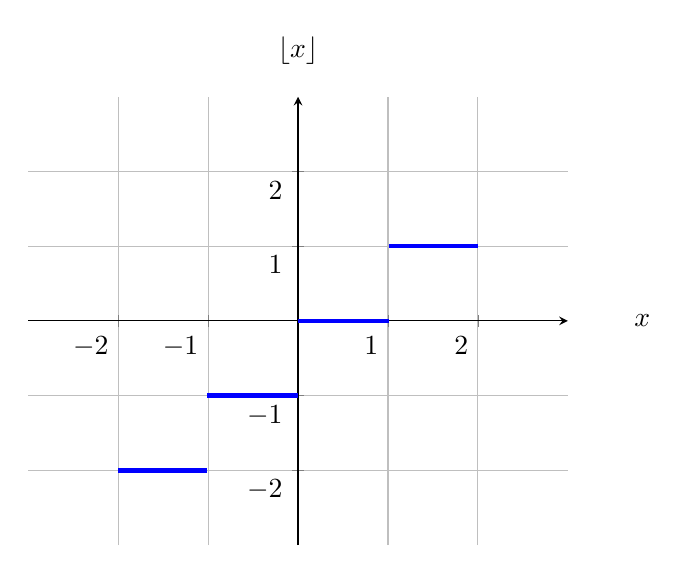
\begin{tikzpicture}
				\begin{axis}[axis lines=middle,
				xtick={-2, -1, 0, 1, 2},
				ytick={-2, -1, 0, 1, 2},
				xticklabel style={below left},
				yticklabel style={below left},
				xmin=-3, xmax=3,
				ymin=-3, ymax=3,
				ylabel={$\lfloor x \rfloor$},
				xlabel={$x$},
				grid,
				every axis x label/.style={
					at={(ticklabel* cs:1.105)},
					anchor= west,
				},
				every axis y label/.style={
					at={(ticklabel* cs:1.05)},
					anchor= south,
				},
				]
				\addplot [
                jump mark mid,
                domain=-2:2,
                samples=100,
                ultra thick, blue
                ] {floor(x)};
				\end{axis}
				\end{tikzpicture}
				\caption{The floor function $\lfloor x \rfloor$ for $-2 \leq x \leq 2$.}
				\label{fig:floorfunction}
			\end{figure}

		\end{definition}

		\begin{example}
			$\lfloor 3.1415\rfloor=3$, $\lfloor-2\rfloor=-2$, and $\lfloor5\rfloor=5$. Figure \ref{fig:floorfunction} shows the value of $\lfloor x \rfloor$ for $x$ between $-2$ and $2$. For positive real numbers, the fractional part is simply the the non-integer part of the number. For example, the fractional part of  $3.14$ is $0.14$. However, the definition of fractional part for negative real numbers may be deceptive. For instance, the fractional part of $-3.14$ is not $0.14$, but
			    \begin{align*}
			        \{-3.14\} &= -3.14 - (-4)\\
			                  &= 0.86.
			    \end{align*}
		\end{example}

	We can generalize the above problem now. The number of integers between two natural numbers $a$ and $b$ (inclusive) which are divisible by $n$ is
		\begin{align*}
		    \left\lfloor\dfrac{b}{n}\right\rfloor-\left\lfloor\dfrac{a-1}{n}\right\rfloor+1
	    \end{align*}
	(Can you see why we are using $a-1$ in the second fraction?) Here, we have assumed that $b\geq a$.

        \begin{proposition}[Properties of Floor Function]\slshape \label{prop:floor}
        	For any two reals $x$ and $y$ and any two integers $m$ and $n$,
        	\begin{enumerate}[1.]
        		\item $x\geq\lfloor x\rfloor>x-1$,
        		%				\item $0 \leq \{x\} <1$,
        		\item if $n \leq x$, then $n \leq \lfloor x \rfloor$,
        		\item $\lfloor x+n\rfloor=\lfloor x\rfloor+n$,
        		\item if $x <y$, then $\lfloor x \rfloor \leq \lfloor y \rfloor$,
        		\item $\lfloor x\rfloor+\lfloor y \rfloor\leq \lfloor x+y\rfloor \leq \lfloor x\rfloor+\lfloor y\rfloor+1$,
        		\item $\lfloor \lfloor x\rfloor\rfloor  =  \lfloor x\rfloor$,
        		\item if $x$ is an integer, $\lfloor x\rfloor+\lfloor -x\rfloor=0$. Otherwise, it equals $1$.
        	\end{enumerate}
        \end{proposition}

        \begin{example}
        	The inequality $\lfloor x\rfloor+\lfloor y\rfloor \leq \lfloor x+y\rfloor$ (as seen in part $5$) is sometimes referred to as the \textit{triangle inequality of floor function}. You can easily check why this inequality holds and find the condition in which it becomes an equality. Put $x=3.6$ and $y=2.5$. Then, $\lfloor x\rfloor+\lfloor y\rfloor = 5$, which is strictly less than $\lfloor x+y\rfloor=6$. The reason why we have a strict inequality here is somewhat obvious now: $0.6$ and $0.5$ add up to $1.1$, which is more than one. You can easily check that only when $\{x\} + \{y\}$ is less than one, the equality case occurs. Otherwise, the inequality is strict.
        \end{example}

        \begin{proof}
        	\begin{enumerate}[1.]
        		\item Let $\lfloor x \rfloor=k$. By definition, $k$ is the greatest integer not exceeding $x$, so $x \geq k$ and $x<k+1$.
        		%				\item This is immediately followed by the first part because $\{x\}=x-\lfloor x \rfloor$. Note that $\{x\}=0$ happens only when $x$ is an integer.
        		\item $n \leq x = \lfloor x \rfloor + \{x\} <\lfloor x \rfloor +1$, and since $n$ is an integer, $n \leq \lfloor x \rfloor$.
        		\item By definition, $\lfloor x \rfloor \leq x$ and so $\lfloor x \rfloor+n \leq x+n$. On the other hand, again by definition, $x < \lfloor x \rfloor+1$. Therefore
        		\begin{align*}
        		\lfloor x \rfloor +n \leq x+n < \lfloor x \rfloor + n+ 1.
        		\end{align*}
        		This means that $\lfloor x \rfloor +n$ is the largest integer less than or equal to $x+n$ and hence $\lfloor x+n\rfloor=\lfloor x\rfloor+n$.
        		\item Write $x<y$ as $\lfloor x \rfloor + \{x\} < \lfloor y \rfloor + \{y\}$ and then $\lfloor x \rfloor < \lfloor y \rfloor +\{y\}-\{x\}$. Now by parts $2$ and $3$,
        		\begin{align*}
        		\lfloor x \rfloor &\leq \bigg\lfloor\lfloor y \rfloor +\{y\}-\{x\}\bigg\rfloor\\
        		&= \lfloor y \rfloor + \bigg\lfloor\overbrace{\{y\}-\{x\}}^{<1}\bigg\rfloor\\
        		&= \lfloor y \rfloor.
        		\end{align*}
        		\item Let $	\lfloor x \rfloor=a, \lfloor y \rfloor=b, \{x\}=a_1$, and $\{y\}=b_1$. By $2$, $a_1, b_1 \geq 0$ and so
        		\begin{align*}
        		a+b \leq a+a_1+b+b_1.
        		\end{align*}
        		Sine $a+b$ is an integer, applying part $2$ we find
        		\begin{align*}
        		\lfloor x \rfloor + \lfloor y \rfloor &= a+b \\
        		&\leq \lfloor a+a_1+b+b_1 \rfloor\\
        		&= \lfloor x+y \rfloor.
        		\end{align*}
        		On the other hand, by part $3$ we observe that
        		\begin{align*}
        		\lfloor x+y \rfloor &= \lfloor a+a_1+b+b_1 \rfloor\\
        		&= a + b + \lfloor a_1+b_1 \rfloor\\
        		&= \lfloor x \rfloor + \lfloor y \rfloor + \lfloor \overbrace{a_1+b_1}^{<2} \rfloor\\
        		&\leq \lfloor x \rfloor + \lfloor y \rfloor + 1.
        		\end{align*}

        		\item $\lfloor x\rfloor$ is an integer and the floor of every integer is equal to itself.
        		\item This is immediately implied from definition.
        	\end{enumerate}
        \end{proof}

	    \begin{proposition}[Properties of Fractional Part]
	    	For any real $x$,
	    	\begin{enumerate}[1.]
	    		\item $0\leq\{x\}<1$,
	    		\item  $\{ x+n\}=\{ x\}$,
	    		\item $\{\{x\}\} =  \{x\}$,
	    		\item if $x$ is an integer, $\{ x\}+\{ -x\}$ is zero, otherwise it equals $1$.
	    	\end{enumerate}
	    \end{proposition}

	    Proofs are straightforward and we leave them for the reader as an exercise.


    Now, we get to the other way of solving problem \ref{floorproblem}. First, we subtracted the number of multiples less than $10$. This time we find out the first multiple of $7$ that is \textit{greater than or equal to} $10$, and the greatest multiple less than or equal to $100$ (this part is same as before). $14=7\cdot2$ is the first multiple of $7$ greater than $10$. Since $98=7\cdot14$ is the largest multiple of $7$ less than $100$, the answer to the problem would be the number of integers between $2$ and $14$ (inclusive). There are $14-2+1=13$ such integers. Consequently, this makes us define \textit{ceiling}. Try to make sense how this relates to the properties of this function.

        \begin{definition}[\bfseries Ceiling Function]
        	We call the function $\lceil x \rceil: \mathbb{R} \to \mathbb Z$ the \textit{ceiling function} and for every real $x$, $\lceil x\rceil$ (read \textit{ceiling of $x$}) is the smallest integer greater than or equal to $x$.

    		\begin{figure}
    			\centering
    			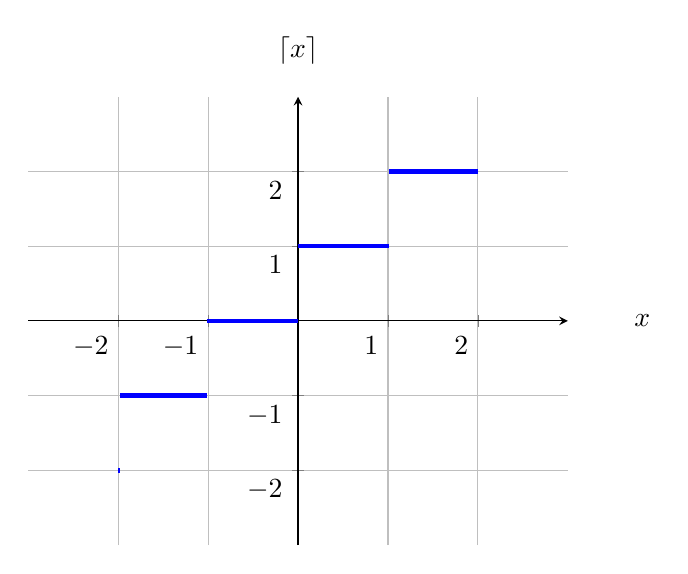
\begin{tikzpicture}
    			\begin{axis}[axis lines=middle,
    			xtick={-2, -1, 0, 1, 2},
    			ytick={-2, -1, 0, 1, 2},
    			xticklabel style={below left},
    			yticklabel style={below left},
    			xmin=-3, xmax=3,
    			ymin=-3, ymax=3,
    			ylabel={$\lceil x \rceil$},
    			xlabel={$x$},
    			grid,
    			every axis x label/.style={
    				at={(ticklabel* cs:1.105)},
    				anchor= west,
    			},
    			every axis y label/.style={
    				at={(ticklabel* cs:1.05)},
    				anchor= south,
    			},
    			]
    			\addplot [
    			jump mark mid,
    			domain=-2:2,
    			samples=100,
    			ultra thick, blue
    			] {ceil(x)};
    			\end{axis}
    			\end{tikzpicture}
    			\caption{The ceiling function $\lceil x \rceil$ for $-2 \leq x \leq 2$.}
    			\label{fig:ceilingfunction}
    		\end{figure}
    	\end{definition}

    	\begin{example}
    		$\lceil3.14\rceil=4$ and $\lceil4\rceil=4$. Also $\lceil-4.1\rceil=-4$ whereas $\lceil4.1\rceil=5$. As seen in figure \ref{fig:ceilingfunction}, similar to the floor function, the plot of the ceiling is like a chain of steps. Every two real numbers which lie between two consecutive integers have the same ceiling and floor value. Compare the plots of these two functions.
    	\end{example}

        \begin{proposition}[Properties of Ceiling Function]\slshape \label{prop:ceiling}
        	For any two reals $x, y$ and any two integers $m,n$,
        	\begin{enumerate}[1.]
        		\item $x\leq \lceil x\rceil < x+1$,
        		\item if $n \geq x$, then $n \geq \lceil x \rceil$,
        		\item $\lceil x+n\rceil=\lceil x\rceil+n$,
        		\item if $x <y$, then $\lceil x \rceil \leq \lceil y \rceil$,
        		\item $\lceil x\rceil+\lceil y \rceil - 1 \leq \lceil x+y\rceil \leq \lceil x\rceil+\lceil y\rceil$,
        		\item $\lceil \lceil x\rceil\rceil  =  \lceil x\rceil$,
        		\item if $x$ is an integer, $\lceil x\rceil+\lceil -x\rceil=0$. Otherwise, it equals $1$,
        		\item $\lceil x \rceil \geq x \geq \lfloor x \rfloor$.
        	\end{enumerate}
        \end{proposition}

    The proofs are pretty much the same as those of floor function and we do not provide them here.

        \begin{problem}\slshape\label{thm:floor-k|n+1}
        	For any two positive integers $n$ and $k$, the following equation holds
        	\begin{align*}
        	\left\lfloor \frac{n+1}{k} \right\rfloor - \left\lfloor \frac{n}{k} \right\rfloor &=
        	\begin{cases}
        	1&\mbox{if }k|n+1,\\
        	0&\mbox{otherwise.}
        	\end{cases}\\
        	\left\lfloor \frac{n+1}{k} \right\rfloor^2 - \left\lfloor \frac{n}{k} \right\rfloor^2 &=
        	\begin{cases}
        	2\frac{n+1}{k}-1&\mbox{if }k|n+1,\\
        	0&\mbox{otherwise.}
        	\end{cases}
        	\end{align*}
        \end{problem}

    \begin{solution}
    	We will prove the first identity. The second one can be proved in a similar way. Let $n+1=kq+r$ for some positive integers $q$ and $r$ such that $0 \leq r <k$. Then,
    	\begin{align*}
    	\left\lfloor \frac{n+1}{k} \right\rfloor - \left\lfloor \frac{n}{k} \right\rfloor &=\left\lfloor \frac{kq+r}{k} \right\rfloor - \left\lfloor \frac{kq+r-1}{k} \right\rfloor\\
    	&= \left\lfloor q+\frac{r}{k} \right\rfloor - \left\lfloor q+\frac{r-1}{k} \right\rfloor\\
    	&= \left(q+\left\lfloor \frac{r}{k} \right\rfloor\right) - \left(q+\left\lfloor \frac{r-1}{k} \right\rfloor\right)\\
    	&= \left\lfloor \frac{r}{k} \right\rfloor - \left\lfloor \frac{r-1}{k} \right\rfloor.
    	\end{align*}
    	Now, since $r<k$, if $r \neq 0$, both $\lfloor r/k \rfloor$ and $\lfloor (r-1)/k \rfloor$ are zero and so is their difference. However, when $r=0$, we have $\lfloor r/k \rfloor=0$ and $\lfloor (r-1)/k \rfloor=-1$ and in this case,
    	\begin{align*}
    	\left\lfloor \frac{n+1}{k} \right\rfloor - \left\lfloor \frac{n}{k} \right\rfloor = 1.
    	\end{align*}
    	The proof is complete.
    \end{solution}

    \subsection{Fractions and Increasing Functions}
    \begin{theorem}\slshape
    	Let $x$ be a real number. Then for every positive integers $n$ and any integer $m$,
    	\begin{align*}
    	\bigg\lfloor \frac{x+n}{m}\bigg\rfloor = \bigg\lfloor \frac{\lfloor x \rfloor+n}{m}\bigg\rfloor \quad \text{and} \quad \bigg\lceil \frac{x+n}{m}\bigg\rceil = \bigg\lceil \frac{\lceil x \rceil+n}{m}\bigg\rceil.
    	\end{align*}
    \end{theorem}

\begin{proof}
	We only show the equality occurs for floor function. The proof for ceiling function is almost the same and is left as an exercise to the reader. Let $f: \mathbb{R} \to \mathbb{R}$ be a function defined by $f(x)=(x+n)/m$. We want to show that $\lfloor f(x) \rfloor = \lfloor f(\lfloor x \rfloor) \rfloor$. We know that $\lfloor x \rfloor \leq x$. If $\lfloor x \rfloor = x$ (i.e., if $x$ is an integer) there is nothing to prove. So, suppose that $\lfloor x \rfloor < x$. The function $f(x)$ is strictly increasing. That is, if $x_1<x_2$ for two reals $x_1$ and $x_2$, then $f(x_1) < f(x_2)$. Therefore $\lfloor x \rfloor < x$ implies $f(\lfloor x \rfloor) < f(x)$. Now by part $4$ of proposition \ref{prop:floor},
	\begin{align*}
	\bigg\lfloor f(\lfloor x \rfloor)\bigg\rfloor  \leq \bigg\lfloor f(x) \bigg\rfloor.
	\end{align*}
	We will show that $\lfloor f(\lfloor x \rfloor)\rfloor  < \lfloor f(x) \rfloor$ does not happen. Suppose on the contrary that it does happen. Let $k =  \lfloor f(x) \rfloor$ and $y=km-n$. Then,
	\begin{align*}
	f(y) &= \dfrac{y+n}{m}\\
	&= \dfrac{(km-n)+n}{m}\\
	&= k\\
	&= \lfloor f(x) \rfloor.
	\end{align*}
	So $f(y)=\lfloor f(x) \rfloor \leq f(x)$, which implies $y \leq x$ (because $f$ is strictly increasing). Also, $y > \lfloor x \rfloor$ because otherwise $\lfloor f(x) \rfloor = f(y) \leq  f(\lfloor x \rfloor)$ and by part $2$ of proposition \ref{prop:floor}, $\lfloor f(x) \rfloor \leq \lfloor f(\lfloor x \rfloor)\rfloor$, which is in contradiction with our assumption. This means that we have found an integer $y$ such that $\lfloor x \rfloor < y \leq x$. This is obviously in contradiction with the definition of $\lfloor x \rfloor$ (since $x$ is non-integer). Therefore, $\lfloor f(x) \rfloor = \lfloor f(\lfloor x \rfloor) \rfloor$ and we are done.
\end{proof}

\begin{corollary}
	For any given real numbers $x, a_1, a_2, \ldots, a_n$, we have
	\begin{align*}
	\Bigg\lfloor \ldots \Big\lfloor \big\lfloor x/a_1 \big\rfloor/a_2 \Big\rfloor \ldots/a_n \Bigg\rfloor &= \Bigg\lfloor \dfrac{x}{a_1a_2\ldots a_n}\Bigg\rfloor, \quad \text{and}\\
	\Bigg\lceil \ldots \Big\lceil \big\lceil x/a_1 \big\rceil/a_2 \Big\rceil \ldots/a_n \Bigg\rceil &= \Bigg\lceil \dfrac{x}{a_1a_2\ldots a_n}\Bigg\rceil.
	\end{align*}
\end{corollary}

The above theorem can be generalized in this way:
\begin{theorem}
	Let $f$ be any continuous and strictly increasing function with the property that if $f(x)$ is an integer, then so is $x$. Then,
	\begin{align*}
	\bigg\lfloor f(\lfloor x \rfloor)\bigg\rfloor  = \bigg\lfloor f(x) \bigg\rfloor \quad \text{and} \quad \bigg\lceil f(\lceil x \rceil)\bigg\rceil  = \bigg\lceil f(x) \bigg\rceil.
	\end{align*}
\end{theorem}

\begin{problem}
	Prove that for every positive real $x$, the following relations hold
		\begin{align*}
		\big\lfloor \sqrt {\lfloor x \rfloor} \big\rfloor &= \lfloor x \rfloor, \quad \text{and}\\
		\big\lceil \sqrt{ \lceil x \rceil} \big\rceil &= \lceil x \rceil.
		\end{align*}
\end{problem}




\subsection{Power of a Prime in a Number} \label{sec:powerofprimes}
In a lot of cases, it just happens that we need to calculate the highest power of a prime $p$ that divides an integer $n$. We denote this by $v_p(n)$. Determining how many zeros there are at the end of $n!$ is a famous problem. Clearly, the number of zeros at the end of any number equals the highest power of $10$ which divides that number, and this is an example of where we need to use this function.

\begin{definition}\label{def:vp}
	We define $v_p(x)$ to be the greatest power in which a prime $p$ divides $x$. In particular, if $v_p(x)=\alpha$, then $p^{\alpha} \mid x$ but $p^{\alpha+1} \nmid x$. We also write $p^{\alpha} \|  x, $ if and only if $v_p(x) = \alpha$.
\end{definition}

\begin{example}
	The greatest power of $3$ that divides $63$ is $3^2.$ because $3^2=9 \mid 63$ but $3^3 =27 \nmid 63.$
	in particular, $ 3^2 \|  63$ or $v_3(63)=2.$
\end{example}

\begin{example}
	If $p$ and $q$ are two different prime numbers, then $ v_p( p^ \alpha q^ \beta) = \alpha$. This can also be shown as $p^\alpha \|  p^ \alpha q^ \beta$.
\end{example}

\begin{proposition} \label{prop:v_p-rule}
	For any two positive integers $x$ and $y$, and any prime $p$, we have
		\begin{align*}
		v_p(xy)=v_p(x)+v_p(y) \quad \text{and} \quad v_p(x+y)\geq\min\left\{v_p(x),v_p(y)\right\}.
		\end{align*}
\end{proposition}

\begin{proof}
	The first equation follows from the product rule of exponentiation ($a^{s} \cdot a^{t} = a^{s+t}$). To make sense the other equation, you can think of a simple example: take $x=9$ and $y=18$. Obviously, $3^3$ does not divide any of $x$ or $y$, but it divides their sum.
\end{proof}

\begin{note}
	$v_p(0)=\infty$ for all primes $p.$
\end{note}

\begin{theorem}[Legendre's Theorem]\label{thm:legendre}\slshape
	Let $p$ be a prime and $n$ be a positive integer. Then
		\begin{align*}
		v_p(n!) & =\sum_{i=1}^{\infty}\left\lfloor\dfrac{n}{p^i}\right\rfloor
		\end{align*}
\end{theorem}

\begin{proof}
	By definition, $n!$ is the product of first $n$ positive integers. Therefore, by proposition \ref{prop:v_p-rule},
		\begin{align*}
			v_p(n!) = v_p(1) v_p(2) \cdots v_p(n).
		\end{align*}
	This means that we have to find the largest power of $p$ in each of integers $1,2,\cdots, n$. As we were finding a solution for problem \ref{floorproblem}, we found out the answer to the question that ''how many integers between $1$ and $n$ are divisible by $p$?`` The answer is $\lfloor n/p \rfloor$, the first term in the sum. Similarly, there are $\lfloor n/p^2 \rfloor$ numbers among these $n$ numbers which are divisible by $p^2$. It is now clear that $v_p(n!)$ is the sum of $\lfloor n/p \rfloor, \lfloor n/p^2 \rfloor, \lfloor n/p^3 \rfloor, \cdots$. We have chosen the upper bound of infinity since the value these floors will be zero after somewhere. If you want to write a sum which includes only non-zero terms, the upper bound would be $v_p(n)$ (why?).
\end{proof}
There is another way for finding $v_p(n!)$ using bases. Before we state the alternative version of Legendre's theorem, we need a definition.
\begin{definition}
	Let $n$ be a positive integer and let $p$ be a prime number.  We denote by $s_p(n)$  the sum of the standard base $p$ digits of $n$. That is, if $n=(n_k n_{k-1}\ldots n_1 n_0)_p$, then $s_p(n)=n_k+ n_{k-1}+\cdots +n_1+ n_0$.
\end{definition}

\begin{example}
	$10=(20)_5$, and so $s_5(10)=2$.
\end{example}


\begin{theorem}\label{thm:legendrealternative}
	Let $p$ be a prime number and let $n$ be a positive integer. Then
	\begin{align*}
	v_p(n!) & =\frac{n-s_p(n)}{p-1}.
	\end{align*}
\end{theorem}

\begin{proof}
	Assume that the base $p$ representation of $n$ is $(n_k n_{k-1}\ldots n_1 n_0)_p$. So $n=n_kp^k + n_{k-1}p^{k-1} + \cdots + n_1 p +n_0$ and
	\begin{align*}
	\left\lfloor\dfrac{n}{p^i}\right\rfloor &=	\left\lfloor\dfrac{n_kp^k + n_{k-1}p^{k-1} + \cdots + n_1 p +n_0}{p^i}\right\rfloor \\
	&= n_kp^{k-i} + n_{k-1}p^{k-i-1} + \cdots + n_{i+1} p + n_i,
	\end{align*}
	for any integer $1 \leq i \leq k$. Now by Legendre's theorem,
	\begin{align*}
	v_p(n!) & = \sum_{i=1}^{k}\left\lfloor\dfrac{n}{p^i}\right\rfloor\\
	&= \left\lfloor\dfrac{n}{p}\right\rfloor+\left\lfloor\dfrac{n}{p^2}\right\rfloor+\cdots+\left\lfloor\dfrac{n}{p^k}\right\rfloor\\
	&= \ \ \ n_kp^{k-1} + n_{k-1}p^{k-2} + \cdots + n_{2} p + n_1 \\  &\ \ \ + n_kp^{k-2} + n_{k-1}p^{k-3} + \cdots + n_{2}\\ &\ \ \ \ \ \ \ \vdots \qquad\qquad \vdots\\  &\ \ \ + n_kp  \ \ \ \ + n_{k-1} \\&\ \ \ + n_k\\
	&=\sum_{i=1}^k n_i(p^{i-1}+p^{i-2}+\cdots+p+1)\\
	&= \sum_{i=1}^k n_i\frac{p^i-1}{p-1}\\
	&=\displaystyle \frac{\displaystyle \sum\limits_{i=0}^k n_i p^i - \sum\limits_{i=0}^k n_i}{p-1}\\
	&=\frac{n-s_p(n)}{p-1}.
	\end{align*}
\end{proof}

\subsection{Kummer's Theorem}
It may seem difficult to find a relation for the largest power of a prime $p$ that divides a binomial coefficient $\binom{m}{n}$. In $1852$, Kummer published an article in which he introduced a very simple way to find $v_p\left(\binom{m}{n}\right)$.

\begin{theorem}[Kummer's Theorem]
	Let $p$ be a prime and let $m$ and $n$ be positive integers such that $n \leq m$. Take $s$ to be the number of \textit{carries} when $n$ is added to $m-n$ in base $p$. Then $s = v_p\left( \binom{m}{n}\right)$.
\end{theorem}

To make a good sense of this theorem, we provide an example and then move to the proof.

\begin{example}
	Let us find $v_3\left( \binom{28}{11}\right)$. First, find the base-$3$ representation of $11$ and $28-11=17$:
		\begin{align*}
			11 = (102)_3, \quad \text{and} \quad 17 = (122)_3.
		\end{align*}
	Now we do the columnar addition to see how many carries happen when we add $(1001)_3$ and $(122)_3$:
		\begin{center}
			\begin{tabular}{c*{4}{@{\,}c}}
				 &  $\overset{1}{\phantom{1}}$   & $\overset{1}{1}$ & $\overset{1}{0}$ & $2$\\
				+& 		& $1$				   & $2$ 			  	  & $2$\\ \hline
				 & $1$	& $0$				   & $0$ 			      & $1$\\
			\end{tabular}
		\end{center}
	We see that three carries happen. Therefore, Kummer's theorem tells us that $\binom{28}{11}$ is divisible by $3^3$ but not by $3^4$. If we calculate the value of this binomial coefficient, we obtain
		\begin{align*}
			\binom{28}{11} &= 21474180\\
						   &= 2^2 \times 3^3 \times 5 \times 7 \times 13 \times 19 \times 23,
		\end{align*}
	which verifies our result.

Let us prove Kummer's theorem now.

\end{example}
\begin{proof}
	Let the representation of $m, n$, and $m-n$ in base $p$ be
	\begin{align*}
	m   &= m_kp^k+m_{k-1}p^{k-1}+\cdots +m_1p+m_0,\\
	n   &= n_kp^k+n_{k-1}p^{k-1}+\cdots +n_1p+n_0,\\
	m-n &= q_kp^k+q_{k-1}p^{k-1}+\cdots +q_1p+q_0.
	\end{align*}
	Let's find the number of carriers in addition of $m$ and $m-n$ in base $p$. We can write
	\begin{align*}
	q_0+n_0  &= m_0 + x_1 p,\\
	q_1+n_1+x_1&= m_1 + x_2p,\\
	&\phantom{=}\vdots\\
	q_k+n_k+x_k&= m_k,
	\end{align*}
	where $x_i$ denotes the carry at the $(i-1)^{th}$ digit from the right (it's either one or zero). Adding all the above equations, we find
	\begin{align*}
	(q_k+q_{k-1}+\cdots+q_0)+(n_k+n_{k-1}+\cdots+n_0) &= (m_k+m_{k-1}+ \cdots+m_0)\\&+(p-1)(x_k+x_{k-1}+\cdots+x_0).
	\end{align*}
	Therefore, the number of carries in the addition is
	\begin{align*}
	s &= x_k+x_{k-1}+\cdots+x_0 \\
	&= \frac{(q_k+q_{k-1}+\cdots+q_0) + (n_k+n_{k-1}+\cdots+n_0) - (m_k+m_{k-1}+\cdots+m_0)}{p-1}.
	\end{align*}
	We will use the fact that
	\begin{align*}
	v_p\left( \binom{m}{n}\right) &= v_p(m!)-v_p(n!)-v_p((m-n)!)
	\end{align*}
	along with theorem \ref{thm:legendrealternative} to show that $s=v_p\left( \binom{m}{n}\right)$. By theorem \ref{thm:legendrealternative}, we know that for every positive integer $a$,
	\begin{align*}
	v_p(a!) & =\frac{a-s_p(a)}{p-1},
	\end{align*}
	where $s_p(a)$ denotes the sum of the standard base $p$ digits of $a$. Therefore,
	\begin{align*}
	v_p\left( \binom{m}{n}\right) &= \frac{m-s_p(m)}{p-1} - \frac{n-s_p(n)}{p-1} - \frac{(m-n)-s_p(m-n)}{p-1}\\
	&= \frac{m-(m_k+m_{k-1}+\cdots+m_0)}{p-1} \\&\phantom{=}-\frac{n-(n_k+n_{k-1}+\cdots+n_0)}{p-1} \\&\phantom{=}-\frac{(m-n)-(q_k+q_{k-1}+\cdots+q_0)}{p-1}\\
	&= \frac{(q_k+q_{k-1}+\cdots+q_0) + (n_k+n_{k-1}+\cdots+n_0) - (m_k+m_{k-1}+\cdots+m_0)}{p-1}\\
	&=s.
	\end{align*}
	The proof is complete.
\end{proof}

\begin{corollary}\label{cor:kummer-corollary}
	Let $p$ be a prime and let $n$ be a positive integer. For any positive integer $k$ such that $0<k\leq p^n$,
	\begin{align*}
	v_p\left( \binom{p^n}{k}\right)	= n - v_p(k).
	\end{align*}
\end{corollary}

\begin{proof}
	When you add $p^n - k$ and $k$ in base $p$, you get a $1$ followed by $n$ zeros. Starting the addition from the rightmost digits and moving to the left, you get a carry as soon as both digits in the column are not zero. In other words, the first carry happens at the first (rightmost) non-zero of $k$ in base $p$ and you will have a carry for all digits after that. So, we are searching for the rightmost non-zero digit of $k$ in base $p$. This is exactly the $(v_p(k)+1)^{th}$ digit (why?). Thus, the number of carries would be
	\begin{align*}
	(n+1)-(v_p(k)+1) = n-v_p(k),
	\end{align*}
	which is what we wanted.
\end{proof}
\begin{problem}
	Let $p$ be a prime and let $m,n$ be positive integers. If $p^m < n < p^{m+1}$, prove that $v_p\left(\binom{n}{k}\right) \leq m$ for every positive integer $k\leq n$.
\end{problem}

\begin{solution}
	The condition $p^m < n < p^{m+1}$ means that $n$ has $m+1$ digits when represented in base $p$. By Kummer's theorem, $v_p\left(\binom{n}{k}\right)$ is the number of carries in addition $k+(n-k)$ in base $p$. Obviously, the number of carries must be less than number of digits of $n$ in base $p$ (why?). The conclusion follows.
\end{solution}
We will provide another solution for problem \ref{prob:china2015-bertrand} stated in section \ref{sec:bertrand}.

\begin{problem}[China 2015]
	Determine all integers $k$ such that there exists infinitely many positive integers $n$ satisfying
	\begin{align*}
	n+k \not \Big| \binom{2n}{n}.
	\end{align*}
\end{problem}

\begin{solution}
	We already know that $n+1 \big| \binom{2n}{n}$ (see solution of problem \ref{prob:china2015-bertrand}). We will prove that all integers except $k=1$ satisfy the given condition. First, let us handle the case $k=0$. In this case, choose $n=2^m$ for any integer $m\geq 2$. By Kummer's Theorem, $v_2\left(\binom{2n}{n}\right)=1$. On the other hand, $4|n$, thus $	n \not \big| \binom{2n}{n}$.

	For $k \ne 0,1$, take any $m \geq 3 + {\log _2}\left| k \right|$, and choose $n = {2^\alpha } - k$. From Kummer's theorem, $v_2\left(\binom{2n}{n}\right) \leq m - 1$, but $n + k = {2^m}$. That is, $n+k \not \big| \binom{2n}{n}$ for our choice of $n$.
\end{solution}

\begin{problem}
	Let $n$ be a positive integer. Show that $n$ divides $\binom{n}{k}$ for all $k$ such that $1 \leq k \leq n-1$ if and only if $n$ is a prime.
\end{problem}

\begin{solution}
	We will first prove that $n$ must be a power of a prime. Suppose the contrary. Take any prime divisor $p$ of $n$ and let $v=v_p(n)$. By Lucas' theorem, it follows that $p \not\big| \binom{n}{p^v}$, which contradicts the assumption that $n \big| \binom{n}{p^v}$. Thus, $n$ must be a power of a prime.

	Write $n=p^r$ for some prime $p$ and positive integer $r$. if $r>1$, then from corollary \ref{cor:kummer-corollary},
	\begin{align*}
	p^2 \not \Big| \binom{n}{p^{r-1}},
	\end{align*}
	which is a contradiction. Therefore, $r=1$ and $n$ must be a prime.

\end{solution}

\section{Common Arithmetic Functions}
	\subsection{Number of Divisors}\label{sec:number-of-divisors}
		We first introduced $\tau(n)$ in chapter \ref{ch:divisibility}. To be precise, in theorem \ref{thm:nos}, we explained that there are $\tau(n)$ positive integer solutions $(a,b)$ to the equation $ab=n$. For example, $ab=12$ has $\tau(12)=6$ solutions $(1,12), (2, 6), (3,4), (4,3), (6,2), (12,1)$ in positive integers.

			\begin{definition}[\bfseries Number-of-divisors Function]
				Let $n$ be a positive integer. The number of positive divisors of $n$ is denoted by $\tau(n)$. In other words, the \textit{number-of-divisors} function is defined as
					\begin{align*}
						\tau(n)=\sum_{d\mid n} 1.
					\end{align*}
			\end{definition}
		What if the number is so huge that we can not compute all the divisors by hand? Or what if we need to tell a computer how to compute the number of divisors in general?\footnote{Well, you can use a brute force method if you are familiar with programming. But certainly iterating through integers from $1$ to $n$ or a solution of that complexity is not a good idea.} If you need more motivation to find a way to compute number of divisors easily, consider the following nice problem!
			\begin{problem}[Bangladesh National Mathematical Olympiad, $\boldsymbol {2010}$]
				You have a regular $2016$-gon. You have to choose some points from that polygon so that the resulting polygon you get from those points is a regular polygon. How many distinct regular polygons can you construct this way? Order of vertex is not important. And the polygon will be constructed joining a point with the next one in an order that does not result in a self intersecting polygon or a polygon which has an angle larger than $180$ (convex simple polygon in other words).
			\end{problem}

			\begin{solution}
				First, try to make sense of what this problem is asking for. This is one of those problems that makes you think in a nice way while also teaching that theorems are not everything to solve problems. A very important point to keep in mind here is that, the order in which we pick the points does not matter.

				The next step should be finding out how we should pick those points if we want to make a regular polygon. And of course, how many point for that matter. Let us label the points of the $2016$-gon as $P_1,P_2,\ldots,P_{2016}$. So, the regular polygon would be $P_1P_2\ldots P_{2016}$. Here, $P_1$ is connected to $P_2$, $P_2$ to $P_3$, and so on. However, $P_{2016}$ would be connected to $P_1$ to complete the cycle of the polygon.

				An important observation: we can always let $P_1$ be the first vertex of the regular polygon we want to construct. Because no matter where we start from, if we rotate, it would be identical to the one that can be created starting from $P_1$. So, $P_1$ is the first vertex of our regular polygon. Also, we fix the number of points in the new regular polygon we want to create. If it has $k$ points, all $k$ sides must be equal.

				Assume that we want to construct a regular quadrilateral $P_1P_iP_jP_k$. What can we say about $i, j$ or $k$? The length $P_1P_i$ must be equal to $P_iP_j$, and $P_jP_k$. This implies that $j$ must be $i+i$. Because if $j<i$ then $P_iP_j$ would be less than $P_1P_i$ (if you are confused about it, just rotate $P_iP_j$ back to $P_1P_i$). Then we also must have $k=3i$. This in turn implies that if there are $m$ points we must have $2016=mq$ for some integer $q$. That is, $m$ must be a divisor of $2016$. Therefore, the number of distinct polygons is the number of distinct divisors of $2016$. But we must consider divisors greater than $2$ only. Because we can not create a polygon with one or two points. We have found the solution, but it would be a lot nicer if we actually knew the value of that.
			\end{solution}
		We will see how to compute number of divisors for a positive integer $n$. Take $n=12$. If $d$ is a divisor of $n$, then it is evident that $d$ can not have any prime factor that is not in $n$. But the opposite might be true. $n$ might have some prime factor that is not in $d$. In this case, a divisor of $12$ must have prime factor of $2$ and $3$ only. Second observation is: we have $n=2^2\cdot3^1$. Thus, $d$ can not have the exponent of $2$ greater than $2$ or the exponent of $3$ greater than $1$. If $d=2^a3^b$ then $a\leq2$ and $b\leq1$. The most interesting part is that, we can actually generate all the divisors this way. Set $a=0,1,2$ and $b=0,1$. Consider the sets $A=\{2^0,2^1,2^2\}$ and $B=\{3^0,3^1\}$. If we multiply an element of $A$ with an element of $B$, we get a divisor of $12$. And for each multiplication, we get a distinct divisor each time. And certainly, this can be generalized. If the prime factorization of $n$ is $p_1^{e_1}p_2^{e_2}\cdots p_k^{e_k}$, then the divisors can be generated multiplying elements from sets $A_1=\{p_1^0,\ldots,p_1^{e_1}\},A_2=\{p_2^{0},\ldots,p_2^{e_2}\},A_k=\{p_k^0,\ldots,p_k^{e_k} \}$. $A_i$ has $e_i+1$ elements because the exponent ranges from $0$ to $e_1$. Then clearly, the number of divisors of $n$ would be the product of number of elements in all $A_i$, that is, $(e_1+1)\cdots(e_k+1)$. However, we will have to prove something even though it is clear from the example. That is, we will not get a duplicate divisor in this process. This will be left as an exercise for the readers.
			\begin{theorem}\slshape
				Let $n$ be a positive integer with prime factorization $n=p_1^{e_1}p_2^{e_2}\cdots p_k^{e_k}$. Then,
				\begin{align}
				\tau(n) &= \prod_{i=1}^{k} (1+e_i). \label{eq:dformula-eq1}
				\end{align}
			\end{theorem}

			\begin{proof}
				Every positive divisor of $n$ must be of the form
				\begin{align*}
				d = p_1^{\alpha_1} p_2^{\alpha_2} \cdots p_k^{\alpha_k},
				\end{align*}
				where $0 \leq alpha_i \leq e_i$ for $i=1,2,\cdots,k$. There are $e_i+1$ possible values $\{0, 1, 2, \cdots, e_i\}$ for the power of prime $p_i$ in $d$. The number of divisors of $n$, $\tau(n)$, is therefore the product of $e_1+1, e_2+1, \cdots ,$ and $e_k+1$. We are done.
			\end{proof}

			\begin{theorem}\label{prop:tau(n)<2sqrt(n)}
				Let $n$ be a positive integer. Prove that $\tau(n) \leq 2 \sqrt n$.
			\end{theorem}

			\begin{proof}
				We can find two positive integers $a$ and $b$ such that $n=ab$. At least one of $a$ and $b$ is less than or equal to $\sqrt n$ (otherwise their product will be larger than $n$). This means that $\frac{\tau(n)}{2}$ can take at most $\lfloor \sqrt n \rfloor$ values. So,
					\begin{align*}
						\tau(n) \leq 2 \lfloor \sqrt n \rfloor \leq 2 \sqrt n.
					\end{align*}
			\end{proof}

			\begin{theorem}\slshape
				$\tau(n)$ is odd if and only if $n$ is a perfect square.
			\end{theorem}

			\begin{proof}
				Let $n$ be a positive integer with factorization $n=p_1^{e_1}p_2^{e_2}\cdots p_k^{e_k}$ and suppose that $\tau(n)$ is odd. This means that all terms in the right hand side of equation \ref{eq:dformula-eq1} must be odd. Therefore, $e_i$ is even for $i=1,2,\cdots,k$. Take $e_i = 2f_i$ for some integer $f_i$. Then,
					\begin{align*}
						n &= p_1^{e_1}p_2^{e_2}\cdots p_k^{e_k}\\
						&= p_1^{2f_1}p_2^{2f_2}\cdots p_k^{2f_k}\\
						&= \left(p_1^{f_1}p_2^{f_2}\cdots p_k^{f_k}\right)^2,
					\end{align*}
				which is a perfect square. The proof for the converse is easy.
			\end{proof}

			\begin{problem}
				Show that for any integer $n>1$, in the infinite sequence
					\begin{align*}
						n, \tau(n), \tau(\tau(n)), \tau(\tau(\tau(n))),\cdots
					\end{align*}
				all the terms after a certain point onwards are equal to $2$. % Prove that this point is arbitrarily given.
			\end{problem}

			\begin{solution}\footnote{Thanks to Professor Greg Martin for his suggestion about proving $\tau(n)<n$.}

				For $n=2$ the statement is obvious, so assume $n >2$. Note that $\tau(n)$ counts the number of positive integers in the set $\{1,2,\ldots,n\}$ that divide $n$. So, it is at most $n$. For $n>2$, we know that $n-1$ does not divide $n$,  hence $\tau(n) < n$ for all $n>2$. This means that the sequence is strictly decreasing as far as its terms are greater than $2$. The proof is complete.
			\end{solution}
	\subsection{Sum of Divisors}\label{sec:sum-of-divisors}
		The sum of divisors of a number is another important property of each positive integer.

		\begin{definition}[\bfseries Sum-of-divisors Function]
			Let $n$ be a positive integer. The sum of positive divisors of $n$ is denoted by $\sigma(n)$.\footnote{Read ``sigma of $n$''.} In other words, the \textit{sum-of-divisors} function is defined as
			\begin{align*}
			\sigma(n)=\sum_{d\mid n} d.
			\end{align*}
		\end{definition}

		\begin{note}
			One might rephrase this definition as: the sum-of-divisors is the summatory function of $\text{id}$.
		\end{note}

		\begin{example}
			$ $
			\begin{itemize}
				\item $\sigma(p^2) = p^2+p+1$ for any prime $p$.
				\item $\sigma(pq)=pq+p+q+1=(p+1)(q+1)$, for any two primes $p$ and $q$.
			\end{itemize}
		\end{example}



		\begin{note}
			Just like the number-of-divisors function, $\sigma$ is not completely multiplicative. Can you think of an example which shows this?
		\end{note}

		\begin{theorem}\slshape\label{thm:sodfrac}
			For any positive integer $n$,
				\begin{align*}
					\dfrac{\sigma (n)}{n} & = \sum_{d\mid n}\dfrac{1}{d}
				\end{align*}
		\end{theorem}

		\begin{proof}
			Beginning from $\sigma(n) = \sum\limits_{d\mid n} d$, you can simply realize that the equation can be written in the form
			\begin{align*}
			\sigma(n) = \sum_{d\mid n} \frac{n}{d}
			\end{align*}
			because when for every divisor $d$ of $n$, the number $n/d$ also divides $n$. We can now take $n$ out of the sum in the right side of above equation and finish the proof.
		\end{proof}

		\begin{note}
			The idea of employing $n/d$ instead of $d$, where $d$ is a divisor of $n$, is a good trick for solving such problems.
		\end{note}

	As for the case of $\tau(n)$, one can express $\sigma(n)$ explicitly as well.

		\begin{theorem}\slshape \label{thm:sigmaformula}
			Let $n$ be a positive integer with prime factorization $n=p_1^{e_1}p_2^{e_2}\cdots p_k^{e_k}$. Then,
			\begin{align*}
			\sigma(n) &= \prod_{i=1}^{k} \frac{p_i^{e_i+1}-1}{p-1}.
			\end{align*}
		\end{theorem}

		\begin{proof}
			Later in proposition \ref{prop:multiplicative-sigma}, we will show that $\sigma$ is multiplicative. Just accept it for now. So, it suffices to prove the assertion for the case when $n$ is a power of a prime. Let $n=p^\alpha$, where $p$ is a prime and $\alpha$ is a positive integer. In this case, the only divisors of $n$ are $1, p, p^2, \cdots, p^\alpha$. Therefore, their sum, $\sigma(n)$, is
				\begin{align*}
					\sigma(p^\alpha) = 1+p+p^2+\cdots+p^\alpha.
				\end{align*}
			Now, by theorem \ref{id:fatandthin}, we can write the above equation as
				\begin{align*}
					\sigma(p^\alpha) = \frac{p^{\alpha+1} - 1}{p-1}.
				\end{align*}
			To finish the proof, consider any positive integer $n$ with factorization $n=p_1^{e_1}p_2^{e_2}\cdots p_k^{e_k}$. Then,
			\begin{align*}
			\sigma(n) &=  \sigma(p_1^{e_1}p_2^{e_2}\cdots p_k^{e_k})\\
			&= \sigma(p_1^{e_1}) \sigma(p_2^{e_2}) \cdots \sigma(p_k^{e_k})\\
			&= \prod_{i=1}^{k} \frac{p_i^{e_i+1}-1}{p-1}.
			\end{align*}
		\end{proof}

	We are going to define amicable numbers as an application of the sum of divisors function.

	\begin{definition}\label{key}
		Two positive integers are called \textit{amicable numbers}\footnote{Amicable: having a spirit of friendliness.} if the sum of proper divisors of each of them is equal to the other. Recall that a proper divisor of $n$ is a divisor of $n$ which is not equal to $n$. In other words, $(m,n)$ is a pair of amicable numbers if $m=\sigma(n)-n$ and $n=\sigma(m)-m$.
	\end{definition}

	\begin{example}
		The smallest pair of amicable numbers is $(220,284)$. One can easily check this:
		\begin{align*}
			220 &= 1 + 2 +  4 + 71 + 142,\\
			284 &= 1 + 2 + 4 + 5 + 10 + 11 + 20 + 22 + 4 + 55 + 110.
		\end{align*}
	\end{example}

	Amicable numbers have been studied since a very long time ago, and there is evidence that they were known to Pythagoreans (followers of Pythagoras) which originated in the sixth century BC. According to \textcite[Chapter I, Page $39$]{dickson_1952} Th\={a}bit ibn Qurra (826--901) found a formula that generates amicable numbers (which we will state in the following). The Iranian mathematician Muhammad Baqir Yazdi, who lived in 16th century, found the pair $(9363584, 9437056)$ of amicable numbers. You can imagaine how difficult it is to find such numbers without using computers. Over a billion pairs of amicable numbers have been found so far (July 2018).

	\begin{theorem}[Th\={a}bit ibn Qurra's Rule]
		Let $n\geq 2$ be a positive integer such that
		\begin{align*}
			p & = 3 \cdot 2^{n-1} - 1,\\
			q & = 3 \cdot 2^{n} - 1,\\
			r & = 9 \cdot 2^{2n - 1} - 1,
		\end{align*}
		are all primes. Then, $(2^n\cdot p \cdot q,  2^n\cdot r)$ is a pair of amicable numbers.
	\end{theorem}

	\begin{proof}
		Let $a=2^n\cdot p \cdot q$ and  $b=2^n\cdot r$. Since $p, q$, and $r$ are all odd primes, the divisors of $a$ are of the form $2^{\alpha}\cdot p^{\beta} \cdot q^{\gamma}$, where $\alpha, \beta, \gamma $ are integers with $0\leq \alpha \leq n$ and $\beta, \gamma \in \{0, 1\}$. Similarly, the divisors of $b$ are of the form $2^{\delta} \cdot r^{\epsilon}$, where $\delta$ and $\epsilon$ are integers with $0 \leq \delta \leq n$ and $\epsilon \in \{0,1\}$. Hence,
		\begin{align*}
			\sigma(a) &= \sum_{\alpha=0}^{n} \sum_{\beta=0}^{1} \sum_{\gamma=0}^1 2^{\alpha} p^{\beta}  q^{\gamma} = \sum_{\alpha=0}^{n} \sum_{\beta=0}^{1} 2^{\alpha} p^{\beta}   \sum_{\gamma=0}^1 q^{\gamma}   = \sum_{\alpha=0}^{n} \sum_{\beta=0}^{1} 2^{\alpha} p^{\beta}   (q+1) \\
			&= \sum_{\alpha=0}^{n} 2^{\alpha} (q+1) \sum_{\beta=0}^{1} p^{\beta} = \sum_{\alpha=0}^{n} 2^{\alpha} (p+1)(q+1) = (p+1)(q+1)  \sum_{\alpha=0}^{n} 2^{\alpha} \\
			&=  (p+1)(q+1) \left(2^{n+1} - 1\right) = 9 \cdot 2^{2n-1} \left(2^{n+1} - 1\right),
		\end{align*}
		and so,
		\begin{align*}
			\sigma(a)-a =  9 \cdot 2^{2n-1} \left(2^{n+1} - 1\right) - 2^n \left(3 \cdot 2^{n-1} - 1\right) \left(3 \cdot 2^{n} - 1\right) = 2^n \left(9 \cdot 2^{2n-1}-1\right) = b.
		\end{align*}
		We expect the reader to be able to prove $\sigma(b)-b=a$ in a similar way on their own. This shows that $(a,b)$ is a pair of amicable numbers.
	\end{proof}

	The above theorem is pretty interesting, but you might wonder if it gives us all the amicable numbers. The answer is negative. You can compute the values of $p, q, r$, and $a,b$ to see how large they get even when $n$ is as small as $10$. For the above theorem to work, we require $p,q,r$ to be primes, and determining whether those numbers are prime is a difficult task for large $n$.

	The mighty Euler \textcite[Chapter I, Page $42$]{dickson_1952} found a more general formula for amicable numbers and discovered $61$ pairs of amicable numbers at his time. We state Euler's generalization of Th\={a}bit ibn Qurra's rule below, usually called Euler's rule, and leave the proof to the interested reader.

	\begin{theorem}[Euler's Rule]
		Let $m$ and $n$ be positive integers with $m<n$ such that
		\begin{align*}
			p & = 2^m \cdot \left(2^{n-m}+1\right) - 1,\\
			q & = 2^n \cdot  \left(2^{n-m}+1\right)  - 1,\\
			r & = 2^{n+m}\cdot  \left(2^{n-m}+1\right)^2  - 1,
		\end{align*}
		are all primes. Then, $(2^n\cdot p \cdot q,  2^n\cdot r)$ is a pair of amicable numbers.
	\end{theorem}


	\subsection{Euler's and Jordan's Totient Functions}
		We have already defined Euler's totient function and used some of its properties to solve problems. In this section, we will prove those properties and provide some more features of $\varphi$. We already know that $\varphi(n)$ is the number of positive integers less than $n$ which are equal to $n$. Suppose that $n= p_1^{\alpha_1} p_2^{\alpha_2} \cdots p_k^{\alpha_k}$ is the prime factorization of $n$. Then
			\begin{align}
				\varphi(n) & = p_1^{\alpha_1-1} p_2^{\alpha_2-1} \cdots p_k^{\alpha_k-1} \left( p_1 -1 \right) \cdots \left( p_k -1 \right). \label{eq:totientformula}
			\end{align}
		In order to find $\varphi(n)$, we will first find the number of positive integers less than or equal to $n$ which are \textit{not} co-prime to $n$. Then, $\varphi(n)$ would be the difference of this number and $n$. Let us consider the simple case $n=pq$, where $p$ and $q$ are primes. A positive integer less than or equal to $n$ is not co-prime to $n$ if it is divisible by either $p$ or $q$. Let $\psi(n)$ be the number of such positive integers. There are $n/p$ and $n/q$ numbers less than or equal to $n$ which are divisible by $p$ and $q$, respectively. So, we might guess that $\psi(n)=n/p+n/q$. However, notice that we are counting the number $pq$ in both the numbers divisible by $p$ and divisible by $q$. So, the true value for $\psi(n)$ is $n/p+n/q-1$. Thus,
			\begin{align*}
				\varphi(n) &= n - k(n)\\
				&= n - n/p - n/q + 1\\
				&= pq - q - p +1\\
				&= (p-1)(q-1),
			\end{align*}
		which is in agreement with equation \ref{eq:totientformula}. Take another example when $n=p_1,p_2,\cdots,p_k$, where $p_1,p_2,\cdots,p_k$ are different primes. Our first guess for $\psi(n)$ would be $n/p_1 +‌n/p_2 + \cdots + n/p_k$. However, we are counting the numbers divisible by $p_ip_j$ (for $1\leq i <j \leq k$) twice. So, our next guess for $\psi(n)$ is
			\begin{align*}
				\psi(n) &= \sum_{1 \leq i \leq k} \frac{n}{p_i} - \sum_{\substack{1 \leq i < j\leq k }} \frac{n}{p_ip_j}.
			\end{align*}
		But this is still not true. For instance, the number $p_1p_2p_3$ is counted in the first sum and we remove it by subtracting the second sum. So, we would have to add another sum
			\begin{align*}
				\sum\limits_{\substack{1\leq i<j<t\leq k}} \frac{n}{p_ip_jp_t}
			\end{align*}
		to include all products\footnote{Notice the indices under the summation notation} such as $p_1p_2p_3$. This process of adding and subtracting sums is called the \textit{inclusion--exclusion principle}. We will continue the process until we count every number less than or equal to $n$ which is not co-prime to $n$ exactly once. Then, the totient function may be calculated from $\varphi(n) = n - \psi(n)$. The reader is encouraged to calculate $\varphi(n) = (p_1-1)(p_2-1) \cdots (p_k-1)$ using the given approach and check that it is compatible with the formula \ref{eq:totientformula}. The very same approach may be applied to the general case $n= p_1^{\alpha_1} p_2^{\alpha_2} \cdots p_k^{\alpha_k}$ to finally prove formula \ref{eq:totientformula}. We strongly recommend the reader try this method for several examples (e.g., $n=p^2q$ or $n = p^3 q^4r^5$) and then prove the whole thing.

		Using the same method, we can prove a stronger result.

		\begin{theorem}[Generalization of \texorpdfstring{$\boldsymbol{\varphi}$}{\textphi}]
			Let $m$ and $n$ be positive integers and let $n= p_1^{\alpha_1} p_2^{\alpha_2} \cdots p_k^{\alpha_k}$ be the prime factorization of $n$. The number of positive integers less than or equal to $m$ which are co-prime to $n$ is $m - \Psi(m)$, where
			\begin{align*}
			\Psi(m) &= \sum_{1 \leq i_1 \leq k} \left\lfloor\frac{m}{p_{i_1}} \right\rfloor - \sum_{\substack{1 \leq i_1<i_2 \leq k}} \left\lfloor\frac{m}{p_{i_1}p_{i_2}} \right\rfloor + \cdots + (-1)^{k+1} \left\lfloor\frac{m}{p_1p_2\cdots p_k} \right\rfloor.
			\end{align*}
		\end{theorem}
		We already stated (but did not prove) some properties of Euler's totient function in proposition \ref{prop:phiproperties}. Here, we are going to prove them beside a few more.

		\begin{theorem}[Properties of \texorpdfstring{$\boldsymbol{\varphi}$}{\textphi}]\slshape\label{thm:phiproperties-ch:arith}
			Let $m$ and $n$ be positive integers. Then,
				\begin{enumerate}[(a)]
					\item $\varphi$ is a multiplicative function. That is, if $m \bot n$, then
						\begin{align*}
							\varphi(mn)=\varphi(m) \cdot \varphi (n).
						\end{align*}
					\item For all $n \geq 3$, $\varphi(n)$ is even.
					\item $\varphi$ is neither increasing, injective, nor surjective.
					\item If $n$ is factorized as $n= p_1^{\alpha_1} p_2^{\alpha_2} \cdots p_k^{\alpha_k}$, then
						\begin{eqnarray*}
							\varphi(n) & = & n \left( 1 - \frac{1}{p_1} \right)  \left( 1 - \frac{1}{p_2} \right)  \cdots \left( 1 - \frac{1}{p_k} \right)  \\
									   & = & p_1^{\alpha_1-1} p_2^{\alpha_2-1} \cdots p_k^{\alpha_k-1} \left( p_1 -1 \right) \cdots \left( p_k -1 \right).
						\end{eqnarray*}
				\end{enumerate}
		\end{theorem}

		\begin{proof}
			$ $
			\begin{enumerate}[(a)]
				\item Write the numbers $1,2,\cdots,mn$ in a table with $m$ rows and $n$ columns as below:
					\begin{center}
						\begin{tabular}{ccccc}
							$1$ & $m+1$ & $2m+1$ & $\ldots$ & $(n-1)m+1$\\
							$2$ & $m+2$ & $2m+2$ & $\ldots$ & $(n-1)m+2$\\
							$\vdots$ & $\vdots$ & $\vdots$ & $\vdots$ & $\vdots$\\
							$m$ & $2m$ & $3m$ & $\ldots$ & $nm$
						\end{tabular}
					\end{center}
				The numbers in the $r$th row of the table are of the form $km+r$, where $k=0,1,2,\cdots,m-1$. Since $(km+r,m)=(r,m)$, one of these two cases happen: either all numbers in a row are co-prime to $m$ or all of them are not co-prime to $m$. As we are looking for numbers co-prime to $mn$, which are obviously those co-prime to both $m$ and $n$, we consider the rows with all numbers co-prime to $m$. There are $\varphi(m)$ such rows. Consider one such row in th table:
					\begin{center}
						\begin{tabular}{ccccc}
							$r$ & $m+r$ & $2m+r$ & $\ldots$ & $(n-1)m+r$
						\end{tabular}
					\end{center}
				The set $\{0, 1, 2, \cdots, n\}$ is a complete residue system modulo $n$. Since $(m,n)=1$, by proposition \ref{prop:generalcompletesystem} of chapter \ref{ch:congruence}, the numbers in the above row of table also form a complete residue system modulo $n$. This means that all the remainders $0,1,2,\cdots,n-1$ happen when you take the numbers in this row modulo $n$. Now, how many numbers in this row are relatively prime to $n$? The answer is the same number of integers co-prime to $n$ in the set $\{0, 1, 2, \cdots, n\}$, which is $\varphi(n)$ by definition (try to figure out why). Therefore, there are totally $\varphi(m) \cdot \varphi(n)$ numbers in the table which are co-prime to both $m$ and $n$, and hence $mn$. On the other hand, by definition, there are $\varphi(mn)$ numbers co-prime to $mn$. The conclusion follows.

				\item $\varphi(n)$ is the number of positive integers $k$ such that $k \leq n$ and $k \bot n$. The point is that if $k$ is co-prime to $n$, then so is $n-k$. Therefore, for $n\geq 3$, one can match all numbers co-prime to $n$ in pairs of $(k, n-k)$, which means that $\varphi(n)$ must be even.

				\item Take $\varphi(5)>\varphi(6)$, $\varphi(n)=\varphi(2n)$ for all odd $n\geq 1$, and $\varphi(n) \equiv 1 \pmod 2$ as counterexamples.

				\item We have already provided the sketch of a proof in the beginning of this section. Here is another proof using multiplicativity of $\varphi$. Since $\varphi(n)$ is multiplicative, it suffices to prove the result when $n$ is a power of a prime. Let $p$ be a prime and $\alpha \geq 1$ be an integer. The only numbers which are \textit{not} co-prime to $p^\alpha$ between $1,2,\cdots,p^\alpha$ are multiples of $p$. How many multiples of $p$ are there among these numbers? The answer is $p^\alpha/p=p^{\alpha-1}$ (why?). Therefore,
					\begin{align*}
						\varphi(p^\alpha) &= p^\alpha - p^{\alpha -1}\\
						&= p^{\alpha -1} (p-1).
					\end{align*}
				Now, if we factorize $n$ as $p_1^{\alpha_1} p_2^{\alpha_2} \cdots p_k^{\alpha_k}$, we can write
					\begin{eqnarray*}
						\varphi(n) &=& \varphi(p_1^{\alpha_1} p_2^{\alpha_2} \cdots p_k^{\alpha_k})\\
								   &=& \varphi(p_1^{\alpha_1}) \varphi(p_2^{\alpha_2}) \cdots \varphi(p_k^{\alpha_k})\\
								   &=& p_1^{\alpha_1-1} p_2^{\alpha_2-1} \cdots p_k^{\alpha_k-1} \left( p_1 -1 \right) \cdots \left( p_k -1 \right).
					\end{eqnarray*}
			\end{enumerate}
		\end{proof}

		\begin{corollary}\label{cor:phidiv}
			If $a|b$, then $\varphi(a)|\varphi(b)$.
		\end{corollary}

		\begin{theorem}\label{thm:phi*1}
			Prove that
				\begin{align*}
					\sum_{d\mid n} \varphi(d)=n
				\end{align*}
			holds for all positive integers $n$
		\end{theorem}

			Instead of a full proof, we provide an example and the readers  are encouraged to complete the proof for themselves. Let $n=15$ and consider the following $15$ fractions:
				\begin{align*}
					\frac{1}{15},
					\frac{2}{15},
					\frac{3}{15},
					\frac{4}{15},
					\frac{5}{15},
					\frac{6}{15},
					\frac{7}{15},
					\frac{8}{15},
					\frac{9}{15},
					\frac{10}{15},
					\frac{11}{15},
					\frac{12}{15},
					\frac{13}{15},
					\frac{14}{15},
					\frac{15}{15}.
				\end{align*}
			Put all these fractions into lowest terms:
				\begin{align*}
					\frac{1}{15},
					\frac{2}{15},
					\frac{1}{5},
					\frac{4}{15},
					\frac{1}{3},
					\frac{2}{5},
					\frac{7}{15},
					\frac{8}{15},
					\frac{3}{5},
					\frac{2}{3},
					\frac{11}{15},
					\frac{4}{5},
					\frac{13}{15},
					\frac{14}{15},
					\frac{1}{1}.
				\end{align*}
			Obviously, the denominators are all the divisors of $15$. Also, there are $15$ fractions. Now, note that only those fractions whose numerator is relatively prime to $15$ have denominator equal to $15$. These are $$ \frac{1}{15}, \frac{2}{15},\frac{4}{15},\frac{7}{15},\frac{8}{15},\frac{11}{15},\frac{13}{15},\frac{14}{15},$$ which are $\varphi(15)=8$ fractions. Similarly, there are $\varphi(5)=4$ fractions $$ \frac{1}{5},\frac{2}{5},\frac{3}{5},\frac{4}{5} $$ which have denominator equal to $5$, and $\varphi(3)=2$ fractions $$ \frac{1}{3},\frac{2}{3}$$ which have denominator equal to $3$. Therefore, we find that the number of fractions is $15$ on one hand and $\varphi(15)+\varphi(5)+\varphi(3)$ on the other hand. These two must be equal, hence $\varphi(15)+\varphi(5)+\varphi(3)=15$.

	\textit{Camille Jordan} generalized the definition of Euler's totient function and introduced \textit{Jordan's totient functions}.

		\begin{definition}
			Let $n$ and $k$ be positive integers. The number of sequences
				\begin{align*}
					a_1, a_2, \cdots, a_k
				\end{align*}
			of positive integers less than or equal to $n$ such that $(a_1,a_2,\cdots,a_k,n)=1$ is called the \textit{$k^{th}$ Jordan's totient function} and is denoted by $J_k(n)$.
		\end{definition}

		\begin{note}
			Here, $(a_1,a_2,\cdots,a_k,n)$ is the notation for greatest common divisor of all numbers $a_1,a_2,\cdots,a_k$, and $n$.
		\end{note}

		\begin{example}
			$ $
			\begin{itemize}
				\item $J_k(1)=1$ for all positive integers $k$.
				\item Obviously, $J_1(n)=\varphi(n)$. That is, the first Jordan totient function is Euler's totient function.
				\item $J_k(p)=p^k - 1 $ because all positive integers less than $p$ are co-prime to $p$.
				\item Let us write all pairs $(a,b)$ of positive integers less than $6$ such that $(a,b,6)=1$.
					\begin{align*}
						&(1,1), (1,2), (1, 3), (1, 4), (1, 5), (1,6),\\
						&(2,1), (2,3), (2,5),\\
						&(3,1), (3,2), (3,4), (3,5),\\
						&(4,1), (4,3), (4,5),\\
						&(5,1), (5,2), (5,3), (5,4), (5,5), (5,6),\\
						&(6,1), (6,5).
					\end{align*}
				There are $24$ such pairs. Hence, $J_2(6)=24$.
			\end{itemize}
		\end{example}


We will state and prove the properties of Jordan's totient function later in section \ref{sec:euler-jordan}.
\section{Dirichlet Product and M\" {o}bius Inversion}\label{sec:dirichletmobius}
	When working with arithmetic functions, we are mostly interested in the \textit{Dirichlet product} of two functions rather than their normal product. As you keep reading this section, you find out why Dirichlet products are important when studying arithmetic functions.

		\begin{definition}[\bfseries Dirichlet Product or Dirichlet Convolution]
			For two arithmetic functions $f$ and $g$, we define their Dirichlet product as
				\begin{align*}
					h(n)=\sum_{d\mid n}f(d)g\left(\frac nd\right),
				\end{align*}
			where the sum extends over all positive divisors $d$ of $n$. We denote this by $h=f\ast g$. In other words,
				\begin{align*}
					(f\ast g)(n)=\sum_{ab=n}f(a)g(b).
				\end{align*}
		\end{definition}

		\begin{example}
			Let $f$ be the constant $1$ function. Let us find $(f \ast f)(n)$. By definition,
				\begin{eqnarray*}
					(f \ast f)(n) & = & \sum_{d\mid n}f(d)f\left(\frac nd\right)\\
								  & = & \sum_{d\mid n} 1\\
								  & = & \underbrace{1 + 1 + \cdots + 1}_{\text{repeated } \tau(n) \text{ times}}\\
								  & = & \tau(n),
				\end{eqnarray*}
			where $\tau(n)$ is the number of divisors of $n$. More details about this function will be explained in section \ref{sec:d(n)}.
		\end{example}

		\begin{example}
			This time, we aim to find the convolution of constant $1$ function $f$ with the identity function. Again, by definition,
				\begin{eqnarray*}
					(\text{id} \ast f )(n) &=& \sum_{d\mid n}\text{id}(d)f\left(\frac nd\right)\\
									       &=& \sum_{d\mid n} d\\
										   &=& \sigma(n),
					\end{eqnarray*}
			where $\sigma(n)$ is the sum of divisors of $n$. If we show the constant $1$ function by $1(n)$, we can write $(\text{id} \ast 1)(n)=\sigma(n)$ or simply $\text{id} \ast 1 = \sigma$.
		\end{example}

		\begin{proposition}[Properties of Dirichlet Convolution]\slshape \label{prop:convolutionproperties}
			Let $f, g$, and $h$ be any arithmetic functions. The Dirichlet product is
			\begin{enumerate}
				\item \textit{commutative}, that is, $f\ast g = g \ast f$,
				\item \textit{associative}. This means that $(f \ast g) \ast h = f\ast (g\ast h)$,
				\item \textit{distributive}, which means that $f\ast (g+h) = f\ast g+ f\ast h$.
			\end{enumerate}
			Furthermore, the unit function $\varepsilon(n)$ acts as a unit element for Dirichlet product. That is, $\varepsilon\ast f = f \ast \varepsilon = f$ for all arithmetic functions $f$.
		\end{proposition}

		\begin{proof}
			The proof for commutativity of Dirichlet convolution is pretty straightforward using the definition $(f\ast g)(n)=\displaystyle\sum_{ab=n}f(a)g(b)$. Obviously, since there is no difference between $a$ and $b$ in the latter formula, we can write it as
				\begin{eqnarray*}
					(f\ast g)(n) &=& \sum_{ab=n}f(a)g(b)= \sum_{ab=n}f(b)g(a)\\
								 &=& \sum_{ab=n}g(a)f(b)\\
								 &=& (g\ast f)(n).
				\end{eqnarray*}
			Let us prove the associativity property now. By definition,
				\begin{eqnarray*}
					((f \ast g) \ast h)(n) &=& \sum_{cd=n} (f\ast g)(d) h(c)\\
										   &=& \sum_{cd=n} \left(\sum_{ab=d} f(a)g(b)\right) h(c)\\
										   &=& \sum_{cd=n} \left(\sum_{ab=d} f(a)g(b) h(c)\right)\\
										   &=& \sum_{abc=n} f(a)g(b) h(c).
				\end{eqnarray*}
			Again, since there is a symmetry between $a,b$, and $c$, we find that the order of $f,g$, and $h$ in the expression $(f \ast g) \ast h$ does not change the result. Hence, the Dirichlet product is associative.
			The proof for distributivity is similar and is left for the reader. It is also trivial by definition that $\varepsilon$ is the unit element of Dirichlet convolution.
		\end{proof}


		We are going define the M\"{o}bius function $\mu(n)$, which doesn't seem very natural at first sight. As we go deeper in this chapter and in chapter \ref{ch:primes} on primes, we will find out why this is in fact very important. It will help us a lot when solving problems concerning inclusion and exclusion. In other words, the definition of the M\"{o}bius function is natural in the way that it's trying to alternate positive and negative signs in an inclusion-exclusion argument.

		\begin{definition}[\bfseries M\"{o}bius Function]\label{def:mobius}
			The M\"{o}bius function $\mu(n)$ is defined as
				\begin{align*}
					\mu(n) & =
						\begin{cases}
						1&\mbox{ if }n=1,\\
						0&\mbox{ if }n
						\mbox{ is divisible by }p^2
						\mbox{ for some prime }p,\\
						(-1)^k&\mbox{ if }n=p_1p_2\cdots p_k.
						\end{cases}
				\end{align*}
		\end{definition}

		\begin{example}
			$\mu(20)=0$ because $2^2|20$. Also, $\mu(105)=(-1)^3=-1$ since $105=3\cdot5 \cdot 7$. The values of $\mu(n)$ for $n=1,2,\cdots,100$ can be found in table \ref{table:mu(n)}.



			\begin{table}
				\centering
				\begin{tabular}{ | l | l | l | l | l | l | l | l | }
					\hline
					$n$  &
					     $\mu(n)$&
					               $n$  &
					                   $\mu(n)$&
					                            $n$   &
					                                 $\mu(n)$&
					                                            $n$  &
					                                                  $\mu(n)$ \\ \hline
					$1$  & $1$   & $26$ & $1$  & $51$ & $1$  & $76$  & $0$     \\ \hline
					$2$  & $-1$  & $27$ & $0$  & $52$ & $0$  & $77$  & $1$     \\ \hline
					$3$  & $-1$  & $28$ & $0$  & $53$ & $-1$ & $78$  & $-1$    \\ \hline
					$4$  & $0$   & $29$ & $-1$ & $54$ & $0$  & $79$  & $-1$    \\ \hline
					$5$  & $-1$  & $30$ & $-1$ & $55$ & $1$  & $80$  & $0$     \\ \hline
					$6$  & $1$   & $31$ & $-1$ & $56$ & $0$  & $81$  & $0$     \\ \hline
					$7$  & $-1$  & $32$ & $0$  & $57$ & $1$  & $82$  & $1$     \\ \hline
					$8$  & $0$   & $33$ & $1$  & $58$ & $1$  & $83$  & $-1$    \\ \hline
					$9$  & $0$   & $34$ & $1$  & $59$ & $-1$ & $84$  & $0$     \\ \hline
					$10$ & $1$   & $35$ & $1$  & $60$ & $0$  & $85$  & $1$     \\ \hline
					$11$ & $-1$  & $36$ & $0$  & $61$ & $-1$ & $86$  & $1$     \\ \hline
					$12$ & $0$   & $37$ & $-1$ & $62$ & $1$  & $87$  & $1$     \\ \hline
					$13$ & $-1$  & $38$ & $1$  & $63$ & $0$  & $88$  & $0$     \\ \hline
					$14$ & $1$   & $39$ & $1$  & $64$ & $0$  & $89$  & $-1$    \\ \hline
					$15$ & $1$   & $40$ & $0$  & $65$ & $1$  & $90$  & $0$     \\ \hline
					$16$ & $0$   & $41$ & $-1$ & $66$ & $-1$ & $91$  & $1$     \\ \hline
					$17$ & $-1$  & $42$ & $-1$ & $67$ & $-1$ & $92$  & $0$     \\ \hline
					$18$ & $0$   & $43$ & $-1$ & $68$ & $0$  & $93$  & $1$     \\ \hline
					$19$ & $-1$  & $44$ & $0$  & $69$ & $1$  & $94$  & $1$     \\ \hline
					$20$ & $0$   & $45$ & $0$  & $70$ & $-1$ & $95$  & $1$     \\ \hline
					$21$ & $1$   & $46$ & $1$  & $71$ & $-1$ & $96$  & $0$     \\ \hline
					$22$ & $1$   & $47$ & $-1$ & $72$ & $0$  & $97$  & $-1$    \\ \hline
					$23$ & $-1$  & $48$ & $0$  & $73$ & $-1$ & $98$  & $0$     \\ \hline
					$24$ & $0$   & $49$ & $0$  & $74$ & $1$  & $99$  & $0$     \\ \hline
					$25$ & $0$   & $50$ & $0$  & $75$ & $0$  & $100$ & $0$      \\ \hline
				\end{tabular}
				\caption{The M\"{o}bius function values for the first $100$ positive integers.}
				\label{table:mu(n)}
			\end{table}
		\end{example}

	\begin{note}
		Why do we care about M\"{o}bius? We can express long, ugly-looking, tedious sums into a very brief expression including sums over $\mu(n)$. If you feel comfortable with arithmetic functions so far, you might like to see an application of the M\"{o}bius function $\mu(n)$ in theorem \ref{thm:numofprime}. You would be able to make sense of a beautiful application of this function.
	\end{note}
		M\"{o}bius function has amazing properties. The first is that it is multiplicative.
		\begin{proposition}
			The M\"{o}bius function is multiplicative.
		\end{proposition}

		\begin{hint}
			Take $m=p_1^{\alpha_1}p_2^{\alpha_2} \cdots p_k^{\alpha_k}$ and $n=p_1^{\beta_1}p_2^{\beta_2} \cdots p_k^{\beta_k}$ and consider the factorization of the product $mn$. Use the definition of M\"{o}bius function to finish the proof.
		\end{hint}

	You may be wonder why would someone define such a not-very-nice-looking function? What is the motivation behind M\"{o}bius function? In fact, this function is the \textit{inverse} of a specific arithmetic function. Before going further, we must define the Dirichlet inverse of an arithmetic function.

		\begin{definition}[\bfseries Dirichlet Inverse Function]
			Let $f$ be an arithmetic function. The arithmetic function $g$ for which
				\begin{align*}
					f \ast g = \varepsilon
				\end{align*}
			is called the \textit{Dirichlet inverse} of $f$. The function $g$ is often denoted by $f^{-1}$.
		\end{definition}
	You now see why we call $\varepsilon$ the \textit{unit} function. Back to our discussion: let $f$ be an arithmetic function. Compute the Dirichlet product of $f$ and constant $1$ function and let the result be $F$, which is also an arithmetic function. By definition of convolution, we have
		\begin{align*}
			F(n) &= (f\ast 1)(n)\\
			     &= \sum_{d\mid n} f(d).
		\end{align*}
	This function $F$ is called the \textit{summatory function} of $f$. In number theory, there are times when we know what $F=f\ast 1$ is and we want to know what $f$ is. This is where M\"{o}bius function comes in. Suppose that you do not know M\"{o}bius function, and you just define $\mu(n)$ as the Dirichlet inverse of $1(n)$. That is, you define $\mu(n)$ be a function such that $\mu \ast 1 = \varepsilon$. Then, multiply $F$ by $\mu$ and use proposition \ref{prop:convolutionproperties} to get
		\begin{align*}
			F \ast \mu &= (f \ast 1) \ast \mu\\
					   &= f \ast (1 \ast \mu)\\
					   &= f \ast \varepsilon\\
					   &=f.
		\end{align*}
	In other words, you just need to multiply $F$ by $\mu$ to find $f$. So, we just need to find out what our defined function $\mu$ is. A few computations help us find $\mu$, the Dirichlet inverse of $1$. First, $(\mu \ast 1)(1)=\varepsilon(1)=1$, which gives $\mu(1)=1$. Let $p$ be a prime and $\alpha$ be a positive integer. Then,
		\begin{align*}
			(\mu \ast 1)(p^\alpha) &= \varepsilon(p^\alpha)\\
							   &= 0.
		\end{align*}
	On the other hand, by definition of Dirichlet product and using the fact that the only divisors of $p^\alpha$ are $1,p,\cdots,p^\alpha$,
		\begin{align*}
			(\mu \ast 1)(p^\alpha) &= \sum_{d|p^\alpha}\mu(d)\\
							   &= \mu(1) + \mu(p) + \cdots + \mu(p^\alpha)\\
							   &= 0
		\end{align*}
	Since we chose $\alpha$ arbitrarily, the equation $\mu(1) + \mu(p) + \cdots + \mu(p^\alpha)=0$ must be true for all values of $\alpha$. For $\alpha=1$, we find $1 + \mu(p) = 0$, hence $\mu(p)=-1$. Similarly, for $\alpha\geq 2$, we find that $\mu(p^\alpha)=0$. Finally,
		\begin{align*}
			\mu(p^\alpha) & = \begin{cases}
			1&\mbox{ if }\alpha=0,\\
			-1&\mbox{ if }\alpha=1,\\
			0&\mbox{ if }\alpha\geq 2.
			\end{cases}
		\end{align*}
	The general definition of $\mu$, as stated in definition \ref{def:mobius}, can be inferred from the above result using the fact that $\mu$ is a multiplicative function.

	As you can observe, the $\mu$ function is defined to help us find an arithmetic function $f$ given its summatory function $F$. In fact, $f=F \ast \mu$. This was first introduced by M\"{o}bius in $19^{th}$ century and is known as the \textit{M\"{o}bius Inversion Formula}.

		\begin{theorem}[M\"{o}bius Inversion Formula]\slshape
			\label{thm:mobinv}
			If the summatory function of an arithmetic function $f$ is $\displaystyle F(n)=\sum\limits_{d\mid n}f(d)$, then
			\begin{align*}
			f(n) & =\sum_{d\mid n}\mu(d)F\left(\frac nd\right).
			\end{align*}
			In other words, $f=\mu\ast F$.
		\end{theorem}


	When we first discussed Dirichlet inverse of a function, you might have wondered if this inverse always exists. The following theorem sheds light on this issue.

		\begin{theorem}\slshape \label{thm:dirichletinverse}
			For an arithmetic function $f$ with $f(1)\neq0$, the Dirichlet inverse $f^{-1}$ exists and is unique. In fact, $f^{-1}$ can be defined recursively as
				\begin{align*}
				f^{-1}(n) & = \begin{cases}
				\dfrac1{f(1)}&\mbox{ if }n=1,\\ \\
				\displaystyle\dfrac{-1}{f(1)}\sum_{\substack{d\mid n\\d<n}}f^{-1}(d)f\left(\dfrac nd\right)&\mbox{ if }n>1.\\
				\end{cases}
		\end{align*}
		\end{theorem}
	As discussed above, $\mu(n)$ is the Dirichlet inverse of the simplest arithmetic function, $1(n)$. The next theorem follows.
		\begin{theorem}
			\label{thm:mobiusinverse}
			The Dirichlet inverse of the M\"{o}bius function is the constant $1$ function. In other words, $1=\mu^{-1}$ or
			\begin{align*}
			\sum_{d\mid n}\mu(n) & =\varepsilon(n).
			\end{align*}
		\end{theorem}

		\begin{theorem}\slshape\label{thm:sum-of-sum-function}
			Let $f$ be an arithmetic function and denote by $F$ its summatory function. That is, for all positive integers $n$,
				\begin{align*}
					F(n) &= \sum_{d\mid n} f(d).
				\end{align*}
			Then,
				\begin{align*}
					\sum_{k=1}^{n} F(k) &= \sum_{k=1}^{n} f(k) \left\lfloor \frac{n}{k}\right\rfloor.
				\end{align*}
		\end{theorem}

		\begin{proof}
			By definition of $F$, we can write
				\begin{align*}
					\sum_{k=1}^{n} F(k) &= \sum_{k=1}^{n} \sum_{d|k} f(d)\\
										&= \sum_{d|1} f(d) + \sum_{d|2} f(d)\\ &\phantom{=} \qquad \qquad +\cdots + \sum_{d\mid n-1} f(d)+\sum_{d\mid n} f(d).
				\end{align*}
			In the last formula, $f(1)$ is repeated $n$ times because $1$ divides all integers. Also, $f(2)$ is repeated $\lfloor n/2 \rfloor$ times because there are exactly $\lfloor n/2 \rfloor$ numbers between $1$ and $n$ (inclusive) which are even. Analogously, there are exactly $\lfloor n/k \rfloor$ multiples of $k$ ($1 \leq k \leq n$) in this interval and thus $f(k)$ is repeated $\lfloor n/k \rfloor$ times. The proof is complete.
		\end{proof}

		\begin{example}
			According to theorem \ref{thm:mobiusinverse}, the summatory function of $\mu$ is $\varepsilon$. Therefore,
				\begin{align*}
					\sum_{k=1}^{n} \varepsilon(k) &= \sum_{k=1}^{n} \mu(k) \left\lfloor \frac{n}{k}\right\rfloor.
				\end{align*}
			Since $\varepsilon(k)$ equals one when $k=1$ and zero otherwise, the sum on the left side equals one. Consequently,
				\begin{align*}
					\sum_{k=1}^{n} \mu(k) \left\lfloor \frac{n}{k}\right\rfloor = 1.
				\end{align*}
			You can check the correctness of this formula by trying some small values for $n$.
		\end{example}


\section{More on Multiplicative Functions}
The most interesting feature of Dirichlet product is that it preserves multiplicativity. That is, if two arithmetic functions are multiplicative, their Dirichlet product is also multiplicative. Before we prove this, we show a simple case. As we saw in previous sections, the summatory function $F$ of an arithmetic function $f$ is defined by $F=f\ast 1$. So, if $f$ is multiplicative, so is $F$.

		\begin{theorem}\slshape\label{thm:sumfunction}
			Let $n$ be a positive integer with prime factorization $n=p_1^{e_1}p_2^{e_2} \cdots p_k^{e_k}$. If $f$ is a multiplicative function with summatory function $F(n)=\sum\limits_{d\mid n}f(d)$, then
				\begin{eqnarray}
					F(n)
					& = &
					\Big(1+f(p_1)+\ldots+f\left(p_1^{e_1}\right)\Big)\cdots\Big(1+f(p_k)+\ldots+f\left(p_k^{e_k}\right)\Big) \label{eq:multiplicative-eq1}\\
					& = &
					\prod_{i=1}^k\sum_{j=0}^{e_i}f\left(p_i^j\right) \nonumber\\
					& = & \prod_{i=1}^kF\left(p_i^{e_i}\right).\nonumber
				\end{eqnarray}
		\end{theorem}

		\begin{proof}
			The proof somewhat follows from unique prime factorization. Assume $T$ is the expansion of the right side of equation \ref{eq:multiplicative-eq1}.
			If $d$ is a divisor of $n$, then $d=p_1^{w_1}p_2^{w_2}\cdots p_k^{w_k}$, where $0\leq w_i\leq e_i$ for $i=1,2,\cdots,k$. Therefore,
				\begin{eqnarray*}
					f(d)    & = & f\left(p_1^{w_1}p_2^{w_2}\cdots p_k^{w_k}\right)\\
							& = & f\left(p_1^{w_1}\right) f\left(p_2^{w_2}\right)\cdots f\left(p_k^{w_k}\right).
				\end{eqnarray*}
			which is a term that is present in $T$. Thus, we conclude that each term in the sum $F(n)=\sum\limits_{d\mid n}f(d)$ appears in $T$. We can easily find that the converse is also true. After expanding the right side of equation \ref{eq:multiplicative-eq1}, we see that every term in $T$ is of the form
				\begin{align*}
					f\left(p_1^{w_1}\right)	f\left(p_2^{w_2}\right)\cdots f\left(p_k^{w_k}\right),
				\end{align*}
			where $w_i$ are integers with $0 \leq w_i \leq e_i$ for all $i$. Since $f$ is multiplicative, we can write this as
				\begin{align*}
					f\left(p_1^{w_1}p_2^{w_2}\cdots p_k^{w_k}\right),
				\end{align*}
			which equals $f(d)$. Therefore, every term in $T$ is also in $F(n)$. Combining these two, $T=F(n)$.
		\end{proof}



		\begin{corollary}
			If $f$ is a non-zero multiplicative arithmetic function and $n=p_1^{e_1}p_2^{e_2} \cdots p_k^{e_k}$ is the prime factorization of a positive integer $n$,
				\begin{align*}
					\sum\limits_{d\mid n}\mu(d)f(d) = \prod_{i=1}^{k} (1-f(p_i)).
				\end{align*}
		\end{corollary}

		\begin{theorem}[Multiplicative Function Theorem (MFT)] \slshape \label{thm:mft}
			Let $f,g$, and $h$ be arithmetic functions.
				\begin{enumerate}
					\item If $f$ and $g$ are both multiplicative, then so is $f\ast g$.
					\item If $f$ is multiplicative, then so is its Dirichlet inverse.
					\item If $f\ast g$ and $f$ are both multiplicative, then so is $g$.
				\end{enumerate}
		\end{theorem}


		\begin{proof}
			$ $
			\begin{enumerate}
				\item Let $f\ast g=h$. We need to prove that if $a$ and $b$ are co-prime positive integers, $h(ab)=h(a)h(b)$. We have
					\begin{align*}
						h(a)h(b) &= \left[(f\ast g)(a)\right] \cdot \left[(f\ast g)(b)\right]\\
								 &= \sum\limits_{d_1|a}f(d_1)g\left(\frac{a}{d_1}\right)\cdot \sum\limits_{d_2|b}f(d_2)g\left(\frac{b}{d_2}\right)\\
								 &= \sum\limits_{d_1|a, d_2|b}f(d_1)f(d_2)g\left(\frac{a}{d_1}\right)g\left(\frac{b}{d_2}\right)\\
								 &= \sum\limits_{d_1|a, d_2|b}f(d_1d_2)g\left(\frac{ab}{d_1d_2}\right)\\
								 &= \sum\limits_{d|ab}f(d)g\left(\frac{ab}{d}\right)\\
								 &= (f\ast g)(ab)\\
								 &=h(ab),
					\end{align*}
				which is what we wanted.

				\item $f$ is multiplicative, hence $f(mn)=f(m)f(n)$ for all co-prime positive integers $m$ and $n$. Put $m=n=1$ in this equation to get $f(1)=f(1)^2$, which immediately gives $f(1)=1$ because $f$ only accepts positive integer values. Let $g$ be the Dirichlet inverse of $f$. By theorem \ref{thm:dirichletinverse}, $g(1)=1$. We will prove by induction that $g$ is multiplicative. The base case $n=1$ is true. Suppose that $n>1$ and whenever $ab<n$ with $(a,b)=1$, then $g(ab)=g(a)g(b)$. Also, suppose that $xy=n$ with $(x,y)=1$. We will show that $g(xy)=g(x)g(y)$. Since $g$ is the inverse of $f$, we have $(f \ast g)(n) = \varepsilon(n)$. Also, $\varepsilon(n)=0$ for $n>1$. Therefore,
					\begin{eqnarray}
						0 &=& \sum_{d\mid n} f(d) g\left(\frac{n}{d}\right)\nonumber\\
						  &=& \sum_{d|xy} f(d) g\left(\frac{xy}{d}\right) \nonumber\\
						  &=& g(xy) + \sum\limits_{\substack{d|xy \\ d>1}} f(d) g\left(\frac{xy}{d}\right).\label{eq:dirichinverse-eq1}
					\end{eqnarray}
				The sum in equation \ref{eq:dirichinverse-eq1} includes terms of te form $f(d)g(xy/d)$, and since $d$ is larger than $1$, $xy/d$ is less than $xy=n$. Since $x \bot y$, there exist positive integers $d_1$ and $d_2$ such that $d=d_1d_2$, $d_1|x$, and $d_2|y$. As a result,
					\begin{eqnarray*}
						g(xy) &=& - \sum\limits_{\substack{d|xy \\ d>1}} f(d) g\left(\frac{xy}{d}\right)\\
							  &=& - \sum\limits_{\substack{d_1|x, d_2|y \\ d_1d_2>1}} f(d_1d_2) g\left(\frac{x}{d_1} \frac{y}{d_2}\right)\\
							  &=& - \sum\limits_{\substack{d_1|x, d_2|y \\ d_1d_2>1}} f(d_1)f(d_2) g\left(\frac{x}{d_1}\right) g\left(\frac{y}{d_2}\right)\\
							  &=& - \bigg[\sum\limits_{d_1|x, d_2|y} f(d_1)f(d_2) g\left(\frac{x}{d_1}\right) g\left(\frac{y}{d_2}\right)\bigg] + g(x)g(y)\\
							  &=& - \bigg[\underbrace{\sum\limits_{d_1|x} f(d_1) g\left(\frac{x}{d_1}\right)}_{=(f \ast g)(x)} \underbrace{\sum\limits_{d_2|y} f(d_2) g\left(\frac{y}{d_2}\right)}_{=(f \ast g)(y)} \bigg] + g(x)g(y)\\
							  &=& -\left[(f \ast g)(x)\right] \left[(f\ast g)(y)\right] + g(x)g(y).
					\end{eqnarray*}
				So, $g(xy)= -(f \ast g)(x) \cdot (f\ast g)(y) + g(x)g(y)$. Note that since $xy>1$, at least one of $x$ or $y$ is larger than $1$. Therefore, since $g$ is the Dirichlet inverse of $f$, at least one of $(f \ast g)(x)$ or $(f \ast g)(y)$ is equal to zero. Finally, $g(xy)=g(x)g(y)$ and we are done.

				\item Let $f\ast g=h$. Multiply both sides by $f^{-1}$, the Dirichlet inverse of $f$, to get $g = h \ast f^{-1}$ (why?). Multiplicativity of $f$ implies the multiplicativity of $f^{-1}$ by part $2$. Now, from part $1$, since both $h$ and $f^{-1}$ are multiplicative, their product, $g$ must also be multiplicative.
			\end{enumerate}
		\end{proof}

		\begin{note}
			If two functions $f$ and $g$ are \textit{completely} multiplicative, their Dirichlet product is multiplicative, but not necessarily completely multiplicative. An example would be $(1 \ast 1)(n) = \tau(n)$. Although the constant $1$ function is completely multiplicative, the number of divisors function $d$ is not.

			The same is true for part $2$: if $f$ is completely multiplicative, then $f^{-1}$ is multiplicative, but not in general completely multiplicative.
		\end{note}

	In proposition \ref{prop:phiproperties}, we stated that Euler's totient function $\varphi$ is multiplicative. We can now prove this result.

		\begin{proposition}\slshape\label{prop:multiplicativephi}
			Prove that $\varphi$ is multiplicative.
		\end{proposition}

		\begin{proof}
			As proved in theorem \ref{thm:phi*1}, we know that $\varphi \ast 1 = \text{id}$. Obviously, both $1(n)$ and $\text{id}(n)$ are multiplicative. The conclusion follows from part $3$ of theorem \ref{thm:mft}.
		\end{proof}


Although it is not always easy to find the Dirichlet inverse of an arithmetic function, there is an exception for completely multiplicative functions.

		\begin{theorem}[Inverse of Completely Multiplicative Functions]\slshape\label{thm:completelymultiplicative}
			Let $f$ be a multiplicative function. Then $f$ is completely multiplicative if and only if
				\begin{align*}
					f^{-1}(n) = \mu(n) f(n) \quad \text{for all } n \geq 1.
				\end{align*}
		\end{theorem}

		\begin{note}
			Here, $\mu(n)f(n)$ is the \textit{point-wise multiplication} of $\mu$ and $f$ at point $n$. It is not to be confused with Dirichlet product $(\mu \ast f)(n)$.
		\end{note}

		\begin{proof}
			First, if $f$ is completely multiplicative, define $g(n) = \mu(n) f(n)$. Then, by definition of Dirichlet product,
				\begin{eqnarray*}
					(g \ast f)(n) &=& \sum_{d\mid n} g(d) f\left(\frac{n}{d}\right)\\
								  &=& \sum_{d\mid n} \mu(d) f(d) f\left(\frac{n}{d}\right)\\
								  &=& \sum_{d\mid n} \mu(d) f\left(d \cdot \frac{n}{d}\right) \quad \text{since } f \text{ is multiplicative}\\
								  &=& f(n) \sum_{d\mid n} \mu(d)\\
								  &=& f(n) \varepsilon(n) \quad \text{by theorem \ref{thm:mobiusinverse}}\\
								  &=& \varepsilon(n).
				\end{eqnarray*}
			The last equality holds because $f(1)=\varepsilon(1)=1$ (why?) and $\varepsilon(n)=0$ for all $n \geq 2$. This means that $g$ is the Dirichlet inverse of $f$.

			For the converse, suppose that $f^{-1}(n) = \mu(n) f(n)$ and we want to prove that $f$ is completely multiplicative. It suffices to prove that $f(p^\alpha)=f(p)^\alpha$ for every prime $p$ and any positive integer $\alpha$ (why?). We will proceed by induction. The base case $\alpha =1$ is obvious. Suppose that we know $f(p^{\alpha-1})=f(p)^{\alpha-1}$ and we want to show that $f(p^\alpha)=f(p)^\alpha$. For any $n \geq 2$, $(f\ast f^{-1})(n)=\varepsilon(n)=0$. Therefore,
				\begin{align*}
					\sum_{d\mid n} \mu(d) f(d) f\left(\frac{n}{d}\right) &= 0.
				\end{align*}
			Put $n=p^\alpha$ in the above equation to obtain
				\begin{eqnarray*}
					\sum_{d|p^\alpha} \mu(d) f(d) f\left(\frac{n}{d}\right)
						&=& \mu(1)f(1)f(p^\alpha) + \mu(p)f(p)f(p^{\alpha -1}) + \cdots +\mu(p^\alpha) f(p^\alpha)f(1)\\
						&=& \mu(1)f(1)f(p^\alpha) + \mu(p)f(p)f(p^{\alpha -1})\\
						&=& f(p^\alpha) - f(p) f(p^{\alpha -1}) \\
						&=& 0.
				\end{eqnarray*}
			That is, $f(p^\alpha) = f(p) f(p^{\alpha -1})$. Using induction hypothesis, we immediately get the result.
		\end{proof}




\subsection{More on \texorpdfstring{$\boldsymbol{\tau}$}{\texttau(n)}}\label{sec:d(n)}

We provide two proofs for this theorem. The first one uses the concept of multiplicative functions discussed in previous sections. The second solution has a combinatorial spirit.

	\begin{proof}
		Since $d$ is multiplicative, it suffices to find $\tau(n)$ only when $n$ is a power of a prime. Let $n=p^\alpha$ for some prime $p$ and a positive integer $\alpha$. There exist $\alpha+1$ divisors $1, p, p^2, \cdots, p^\alpha$ for $n$. Therefore, $d(p^\alpha)=\alpha + 1$. To prove the theorem in the general case, take $n=p_1^{e_1}p_2^{e_2}\cdots p_k^{e_k}$ and write
			\begin{eqnarray*}
				d(n) &=& d(p_1^{e_1}p_2^{e_2}\cdots p_k^{e_k})\\
					 &=& d(p_1^{e_1}) d(p_2^{e_2})\cdots d(p_k^{e_k})\\
					 &=& (e_1+1)(e_2+1)\cdots (e_k+1)\\
					 &=& \prod_{i=1}^{k} (1+e_i).
			\end{eqnarray*}
	\end{proof}

	\begin{example}
		$ $
		\begin{itemize}
			\item $\tau(p)=2$ for all primes $p$.
			\item $\tau(100) = \tau(2^2 \cdot 5^2) = (2+1)(2+1)=9$.
		\end{itemize}
	\end{example}



	\begin{problem}
		Show that $1 = \tau \ast \mu$.
	\end{problem}

	\begin{solution}
		By theorem \ref{thm:mobiusinverse}, $1 \ast \mu =\varepsilon$. Multiply both sides of this equation by $1$ and use the fact that $1\ast 1 = \tau$, we find
			\begin{eqnarray*}
				\tau \ast \mu &=& 1 \ast 1 \ast \mu \\
							  &=& 1 \ast \varepsilon\\
							  &=& \varepsilon.
			\end{eqnarray*}
	\end{solution}


As mentioned in section \ref{sec:number-of-divisors}, the number of solutions to $ab = n$ in positive integers is $\tau(n)$. For the sake of completeness, we will state this result as a theorem.

	\begin{theorem}\label{thm:ab=n}
		Let $n$ be a positive integer. The number of pairs $(a,b)$ of positive integers which satisfy $ab=n$ is $\tau(n)$.
	\end{theorem}

	\begin{proof}
		First, if for some positive integers $a$ and $b$ the equation $ab = n$ holds, then $a$ is a divisor of $n$. Second, for any divisor $a$ of $n$, the number $b = n/a$ is an integer that satisfies $ab = n$. Therefore, $\tau(n)$ counts exactly all the solutions of $ab=n$.
	\end{proof}


Here is a more interesting question:

	\begin{question}
		Let $x \geq 1$ be a \textit{real} number. Find the number of pairs $(a, b)$ of positive integers which satisfy
			\begin{align}
				ab \leq x. \label{eq:ab<x}
			\end{align}
	\end{question}

One way to answer this question is to break the condition $ab \leq x$ into smaller conditions. Obviously, the equation $ab = y$ does not have any solutions in integers if $y$ is not an integer. So, in order to find the number of solutions to the inequality \ref{eq:ab<x}, we only need to find the number of solutions to each of $ab = 1, ab= 2, \cdots, ab= \lfloor x \rfloor$ and the answer would be the sum of these numbers. According to theorem \ref{thm:ab=n}, the answer is
	\begin{align*}
		\tau(1) + \tau(2) + \cdots + \tau(\lfloor x \rfloor).
	\end{align*}
We are seeking a way to determine this sum.

	\begin{definition}
		Let $x \geq 1$ be a real number. Denote by $T(x)$ the number of positive integer solutions to $ab \leq x$.
	\end{definition}

From what we have already found,
	\begin{align}
		T(x) = \sum_{k=1}^{\lfloor x \rfloor} \tau(k).\label{eq:T(x)-1}
	\end{align}

	\begin{example}
		Let us find $T(10.2)$. We need to compute $\tau(1), \tau(2), \cdots, \tau(10)$.
			\begin{table}
					\begin{center}
						\begin{tabular}{|c|c|}
							\hline
							$n$ & $\tau(n)$\\
							\hline
							$1$ & $1$\\
							\hline
							$2$ & $2$\\
							\hline
							$3$ & $2$\\
							\hline
							$4$ & $3$\\
							\hline
							$5$ & $2$\\
							\hline
							$6$ & $4$\\
							\hline
							$7$ & $2$\\
							\hline
							$8$ & $4$\\
							\hline
							$9$ & $3$\\
							\hline
							$10$ & $4$\\
							\hline
					\end{tabular}
					\caption{Value of $\tau(n)$ for $n=1,2,\cdots,10$.}\label{table:tau}
				\end{center}
			\end{table}
		According to table \ref{table:tau} and equation \ref{eq:T(x)-1}, $T(10.2)$ is equal to the sum of numbers in the second column, which is $27$.
	\end{example}


As you observe in the above example, it would be a tedious job to calculate $T(x)$ by summing up the $\tau$ values. There is another way to compute $T(x)$. Let $a$ be a fixed positive integer. The inequality $ab \leq x$ is equivalent to
	\begin{align*}
		b \leq \frac{x}{a}.
	\end{align*}
Since $b$ is a positive integer, it can take the values $1, 2, \cdots, \lfloor \frac{x}{a}\rfloor$. These are $\lfloor \frac{x}{a}\rfloor$ numbers. Since $a$ can take all the values $1, 2, \cdots, \lfloor x \rfloor$, we have
	\begin{align*}
		T(x) = \left\lfloor \frac{x}{1}\right\rfloor + \left\lfloor \frac{x}{2}\right\rfloor + \cdots + \left\lfloor \frac{x}{\lfloor x \rfloor}\right\rfloor.
	\end{align*}

	\begin{example}
		Let us calculate $T(10.2)$ with the new approach. We have
			\begin{eqnarray*}
				T(10.2) &=& \left\lfloor \frac{10.2}{1}\right\rfloor + \left\lfloor \frac{10.2}{2}\right\rfloor + \cdots + \left\lfloor \frac{10.2}{10}\right\rfloor\\
						&=& 10 + 5 + 3 + 2 + 2 + 1 + 1 + 1 + 1 + 1\\
						&=& 27,
			\end{eqnarray*}
		which is in agreement with our previous result.
	\end{example}

The formula
	\begin{align}
		T(x) = \sum_{k=1}^{\lfloor x \rfloor} \left\lfloor \frac{x}{k} \right\rfloor \label{eq:T(x)-2}
	\end{align}
is more convenient than \ref{eq:T(x)-1}. That is, we can find $T(x)$ using equation \ref{eq:T(x)-2} with less number of calculations. In fact, to compute $T(x)$ from \ref{eq:T(x)-1}, we need to calculate the number of divisors of $\lfloor x \rfloor$ numbers, which obviously needs more computations than $\lfloor x \rfloor$  computations needed in formula \ref{eq:T(x)-2}. However, this can be refined even more.

We will divide the solutions to $ab \leq x$ into two classes. The first class includes solutions in which $a \leq \sqrt x$ and the second one includes all solutions such that $a > \sqrt x$. Let $T_1(x)$ be the number of solutions in the first class and let $T_2(x)$ be that of the second class. Therefore,
	\begin{align*}
		T(x) = T_1(x) + T_2(x).
	\end{align*}

For the first class of solutions, let us consider $1 \leq a \leq \sqrt x$ is a fixed integer. The inequality $ab \leq x$, can be written as $b \leq \frac{x}{a}$. Therefore, in order to satisfy $ab \leq x$, $b$ can take only the values $1, 2,\cdots,\lfloor \frac{x}{a}\rfloor$, which are $\lfloor \frac{x}{a}\rfloor$ different numbers. Keeping in mind that $a$ can take the values $1, 2, \cdots, \lfloor \sqrt x \rfloor$, the number of solutions in the first class is
	\begin{align*}
		T_1(x) &= \sum_{a=1}^{\lfloor\sqrt x\rfloor} \left\lfloor\frac{x}{a}\right\rfloor.
	\end{align*}
For the second class, we must find how many pairs $(a,b)$ of integers satisfy the following inequalities:
	\begin{align*}
		ab \leq x \quad \text{and} \quad a > \sqrt x.
	\end{align*}
This can be written as
	\begin{align*}
		\sqrt x < a \leq \frac{x}{b}.
	\end{align*}
Obviously, since the product of $a$ and $b$ is less than or equal to $x$ and $a > \sqrt x$, we must have $b \leq \sqrt x$ (otherwise $ab$ would be larger than $x$). Fix $b$. The only possible values for $a$ are
	\begin{align*}
		\lfloor \sqrt x \rfloor +1, \lfloor \sqrt x \rfloor +2, \cdots, \left\lfloor \frac{x}{b}\right\rfloor.
	\end{align*}
These are $\lfloor \frac{x}{b}\rfloor - \lfloor \sqrt x \rfloor$ numbers. So, since $b$ can take all values $1, 2, \cdots, \lfloor \sqrt x \rfloor$, we have
	\begin{align}
		T_2(x) &= \sum_{b=1}^{\lfloor\sqrt x\rfloor} \left(\left\lfloor\frac{x}{b}\right\rfloor - \lfloor \sqrt x \rfloor\right). \label{eq:T(x)-3}
	\end{align}
In order to add $T_1(x)$ and $T_2(x)$ to obtain $T(x)$, we have to make their summation parameter the same. We already know that changing the summation parameter does not change the value of the sum. Therefore, we can change $b$ to $a$ in equation \ref{eq:T(x)-3} and write $T_2(x)$ as
	\begin{align*}
		T_2(x) &= \sum_{a=1}^{\lfloor\sqrt x\rfloor} \left(\left\lfloor\frac{x}{a}\right\rfloor - \lfloor \sqrt x \rfloor\right).
	\end{align*}
We can now add up $T_1(x)$ and $T_2(x)$ and write
	\begin{eqnarray*}
		T(x) &=&  T_1(x) + T_2(x)\\
			 &=& \sum_{a=1}^{\lfloor\sqrt x\rfloor} \left\lfloor\frac{x}{a}\right\rfloor + \left(\sum_{a=1}^{\lfloor\sqrt x\rfloor} \left(\left\lfloor\frac{x}{a}\right\rfloor - \lfloor \sqrt x \rfloor\right)\right)\\
			 &=& 2\sum_{a=1}^{\lfloor\sqrt x\rfloor} \left\lfloor\frac{x}{a}\right\rfloor - 2\sum_{a=1}^{\lfloor\sqrt x\rfloor} \lfloor\sqrt x\rfloor\\
		     &=& 2\sum_{a=1}^{\lfloor\sqrt x\rfloor} \left\lfloor\frac{x}{a}\right\rfloor - \left(\underbrace{\lfloor \sqrt x \rfloor + \lfloor \sqrt x \rfloor + \cdots +‌\lfloor \sqrt x \rfloor}_{\lfloor \sqrt x \rfloor \text{ times}}\right)\\
		     &=& 2\sum_{a=1}^{\lfloor\sqrt x\rfloor} \left\lfloor\frac{x}{a}\right\rfloor - \lfloor \sqrt x \rfloor^2.
	\end{eqnarray*}
Finally, we have the formula
	\begin{align}
		T(x) &= 2\sum_{a=1}^{\lfloor\sqrt x\rfloor} \left\lfloor\frac{x}{a}\right\rfloor - \lfloor \sqrt x \rfloor^2.\label{eq:T(x)-4}
	\end{align}
Equation \ref{eq:T(x)-4} needs $\lfloor \sqrt x \rfloor$ computations to calculate $T(x)$, which is obviously less than $\lfloor x \rfloor$ computations needed to find $T(x)$ from \ref{eq:T(x)-2}.

	\begin{example}
		We will calculate the number of positive integer solutions to $ab \leq 100.2$. Since $x=100.2$ is large in this case, the best way to calculate $T(x)$ is from formula \ref{eq:T(x)-4}. We find
			\begin{eqnarray*}
				T(100.2) &=& 2\sum_{a=1}^{10} \left\lfloor\frac{100.2}{a}\right\rfloor - 100\\
						 &=& 2\big(100 + 50 + 33 + 25 + 20 + 16 + 14 + 12 + 11 + 10\big) - 100\\
						 &=& 482.
			\end{eqnarray*}
	\end{example}

	\begin{theorem}[An Approximation for Average Value of $\tau(n)$]
		Let $n$ be a positive integer. Prove that
			\begin{align*}
				\frac{\tau(1) + \tau(2) + \cdots + \tau(n)}{n} = \frac{1}{1} + \frac{1}{2} + \cdots + \frac{1}{n} - e,
			\end{align*}
		where $e$ is a number between zero and one.
	\end{theorem}

	\begin{proof}
		Assuming $x=n$, we employ equations \ref{eq:T(x)-1} and \ref{eq:T(x)-2} to write
			\begin{align*}
				\sum_{k=1}^{n} \tau(k) = \sum_{k=1}^{n} \left\lfloor \frac{n}{k} \right\rfloor
			\end{align*}
		The right hand side of the above equation can be written as
			\begin{align*}
				\sum_{k=1}^{n} \left\lfloor \frac{n}{k} \right\rfloor &= \sum_{k=1}^{n} \left(\frac{n}{k} - \left\{ \frac{n}{k} \right\}\right),
			\end{align*}
		where $\{n/k\}$ is the fractional part of $n/k$. Therefore,
			\begin{align}
				\sum_{k=1}^{n} \tau(k) = \sum_{k=1}^{n} \frac{n}{k}  - \sum_{k=1}^{n} \left\{ \frac{n}{k} \right\}. \label{eq:T(x)-5}
			\end{align}
		Dividing both sides of this last equation by $n$, we find
			\begin{align}
			\frac{\sum\limits_{k=1}^{n} \tau(k)}{n} = \sum_{k=1}^{n} \frac{1}{k}  - \frac{\sum\limits_{k=1}^{n} \left\{ \frac{n}{k} \right\}}{n}.
			\end{align}
		We already know that $0 \leq \{n/k\}<1$. Therefore, the second sum in the right hand side of equation \ref{eq:T(x)-5} is between zero and $n$. Therefore,
			\begin{align*}
				0 < \frac{\sum_{k=1}^{n} \left\{ n/k \right\}}{n} < 1
			\end{align*}
		(it is never equal to zero, can you see why?). The proof is complete.
	\end{proof}

	\begin{note}
		This theorem states that the average value of number-of-divisors function (i.e., $[\tau(1) +‌\tau(2) + \cdots + \tau(n)]/n$) is approximately equal to sum of reciprocals of positive integers up to $n$. We represent this as
			\begin{align*}
				\frac{\tau(1) + \tau(2) + \cdots + \tau(n)}{n} \sim \frac{1}{1} + \frac{1}{2} + \cdots + \frac{1}{n}.
			\end{align*}
	\end{note}


\subsection{More on \texorpdfstring{$\boldsymbol{\sigma}$}{\textsigma(n)} and its Generalization}

	Let us prove that $\sigma$ is multiplicative.

	\begin{proposition}\label{prop:multiplicative-sigma}
		The sum-of-divisors function $\sigma$ is a multiplicative arithmetic function.
	\end{proposition}

	\begin{proof}
		If you look more closely, you will observe that
			\begin{eqnarray*}
				\sigma(n) &=& \sum_{d\mid n} d\\
						  &=& \sum_{d\mid n} d \cdot 1\left(\frac{n}{d}\right)\\
						  &=& (\text{id} \ast 1)(n).
			\end{eqnarray*}
		Now, since both $\text{id}$ and constant $1$ function are multiplicative, part $1$ of theorem \ref{thm:mft} implies that $\sigma$ is also multiplicative.
	\end{proof}


	\begin{problem} %http://artofproblemsolving.com/community/q1h547420p3171512
		Prove that for two positive integers $a$ and $b$, if $a\mid b$, then
		\begin{align*}
			\frac{\sigma(a)}{a}\leq \frac{\sigma(b)}{b}.
		\end{align*}
	\end{problem}

	\begin{solution}
		Let $b=\prod\limits_{p|b}p^e$ be the prime factorization of $b$. Then, since $a|b$, the factorization of $a$ would be $a=\prod\limits_{p|b}p^f$ with $0\leq f\leq e$ for each prime $p$ dividing $b$. From theorem \ref{thm:sigmaformula},
		\begin{align*}
			\sigma(b)=\prod_{p|b}\dfrac{p^{e+1}-1}{p-1}\quad \text{and} \quad 	\sigma(a)=\prod_{p|b}\dfrac{p^{f+1}-1}{p-1}.
		\end{align*}
		Thus, we need to show that
		\begin{align*}
			\prod_{p|b}\dfrac{p^{f+1}-1}{p^f(p-1)}
			\leq\prod_{p|b}\dfrac{p^{e+1}-1}{p^e(p-1)}.
		\end{align*}
		Now it suffices to prove that

		\begin{flalign*}
			&& \dfrac{p^{e+1}-1}{p^e(p-1)} &\geq\dfrac{p^{f+1}-1}{p^f(p-1)} &\\
			\iff && p^{e+f+1}(p-1)-p^f(p-1) &\geq p^{e+f+1}(p-1)-p^e(p-1) & 	\phantom{\iff}\\
			\iff && p^e(p-1) &\geq p^f(p-1),
		\end{flalign*}
		which is true since $e \geq f$.

	\end{solution}

	\begin{proposition}\label{prop:sigma(n)>n+sqrt(n)}
		Let $n$ be a composite positive integer. Prove that $\sigma(n) > n + \sqrt n$.
	\end{proposition}

	\begin{proof}
		Since $n$ is composite, we know from proposition \ref{factorsqrt} that $n$ has a prime factor $p$ less than or equal to $\sqrt n$. Then, $n/p$ is a divisor of $n$ and $n/p \geq \sqrt n$. Since $n$ has at least three divisors $n$, $n/p$, and $1$,
			\begin{eqnarray*}
				\sigma(n) &\geq& n + \frac{n}{p} + 1\\
						  &\geq& n + \sqrt n + 1\\
						  &>& n+ \sqrt n.
			\end{eqnarray*}
	\end{proof}


	\begin{theorem}
		Let $k>1$ be a given positive integer. Show that the equation
			\begin{align*}
				\sigma(n) = n + k
			\end{align*}
		has a finite number of solutions for $n$.
	\end{theorem}

	\begin{proof}
		Suppose that $\sigma(n)=n+k$ holds for some positive integer $n$. Since $k>1$, $n$ must be composite (otherwise $\sigma(n)=n+1$). According to theorem \ref{prop:sigma(n)>n+sqrt(n)}, $\sigma(n) > n + \sqrt n$. As a result, we find $\sqrt n < k$ or $n < k^2$. Obviously, there are at most $k^2$ values $1,2,\cdots,k^2$ possible for $n$. This finishes the proof.
	\end{proof}


	\begin{theorem}
		Let $k$ be an arbitrary positive integer. Show that there exists a positive integer $n_0$ such that for any $n>n_0$,
			\begin{align*}
			\frac{\sigma(n!)}{n!} > k.
			\end{align*}
		In other words, prove that $\lim\limits_{n \to \infty} \frac{\sigma(n!)}{n!}= \infty$.
	\end{theorem}

	\begin{proof}
		According to theorem \ref{thm:sodfrac},
			\begin{align*}
				\frac{\sigma(n!)}{n!} &= \sum_{d\mid n!} \frac{1}{d}.
			\end{align*}
		Since $1,2,\cdots,n$ all divide $n!$, we can write
			\begin{eqnarray*}
				\frac{\sigma(n!)}{n!} &=& \sum_{d\mid n!} \frac{1}{d}\\
									  &>& \frac{1}{1} + \frac{1}{2}+ \cdots + \frac{1}{n}.
			\end{eqnarray*}
		It suffices to find an $n$ such that
			\begin{align*}
				\frac{1}{1} + \frac{1}{2}+ \cdots + \frac{1}{n} > k.
			\end{align*}
		Take $n=2^{2k}$. Then,
			\begin{eqnarray*}
				\frac{1}{1} + \frac{1}{2}+ \cdots + \frac{1}{2^{2k}}
					&>& 1 + \frac{1}{2} + \left(\frac{1}{4} + \frac{1}{4}\right) + \left(\frac{1}{8} + \frac{1}{8}+\frac{1}{8} + \frac{1}{8}\right)\\
					&\phantom{>}& \qquad  + \cdots + \left(\underbrace{\frac{1}{2^{2k}}+\frac{1}{2^{2k}}+\cdots+\frac{1}{2^{2k}}}_{2^{2k-1} \text{ times}}\right)\\
					&>& 1+2k\left(\frac{1}{2}\right)\\
					&=& 1+k\\
					&>& k,
			\end{eqnarray*}
		as desired.
	\end{proof}

	\begin{theorem}\slshape\label{thm:oddsigma}
		$\sigma (n)$ is odd if and only if $n=k^2$ or $n=2k^2$ for some integer $k$.
	\end{theorem}

	\begin{proof}
		Let $n=p_1^{e_1}p_2^{e_2}\cdots p_k^{e_k}$ be the factorization of $n$ and suppose that $\sigma(n)$ is odd. We will prove that $n$ is either a perfect square or twice a perfect square. According to theorem \ref{thm:sigmaformula}, since $\sigma(n)$ is odd, all the terms in the product $\prod\limits_{i=1}^{k} \frac{p_i^{e_i+1}-1}{p-1}$ must be odd. That is,
		\begin{align}
			1+p_i+p_i^2+\cdots+p_i^{e_i} \label{eq:sigma-eq1}
		\end{align}
		must be odd for $i=1,2,\cdots,k$. There are two cases: if $p_i\neq 2$ for all $i$, then the number of terms in the expression \ref{eq:sigma-eq1} must be odd so that their sum is also odd (they are all odd). That is, $e_i$ must be even for $i=1,2,\cdots,k$. Hence, $n$ is a perfect square.

		The other case is when some $p_i$, say $p_1$ is equal to $2$. The expression \ref{eq:sigma-eq1} is odd for $p_1=2$. Now, in order for expression \ref{eq:sigma-eq1} to be odd, all $e_i$ must be even for $2 \leq i \leq k$ (exactly like the previous case). Now, if the power of $2$ that divides $n$ is even, $n$ is of the form $k^2$ and if it is odd, $n$ is of the form $2k^2$.

		The proof of the converse is now obvious.
	\end{proof}

	\begin{corollary}
		If $n$ is an odd positive integer, then $n$ is a square if and only if $\sigma (n)$ is odd.
	\end{corollary}

	\begin{proposition}\slshape
		Let $n$ be a positive integer. The number of positive integers less than or equal to $n$ with even sum of divisors is
		\begin{align*}
			n-\left\lfloor\sqrt{n}\right\rfloor-\left\lfloor\sqrt{\dfrac{n}{2}}\right\rfloor.
		\end{align*}
	\end{proposition}

	\begin{proof}
		There are $n$ positive integers less than or equal to $n$. We know from theorem \ref{thm:oddsigma} that numbers which are a perfect square or twice a perfect square have an even $\sigma$. The number of perfect squares less than or equal to $n$ is $\left\lfloor\sqrt{n}\right\rfloor$ (why?). Similarly, the number of integers less than or equal to $n$ which are twice a perfect square is $\lfloor\sqrt{n/2}\rfloor$. The conclusion follows.
	\end{proof}

	A family of numbers which are related to sum-of-divisors function are \textit{perfect numbers}.

	\begin{definition}
		A positive integer $n$ is a \textit{perfect number} if $\sigma(n)=2n$.
	\end{definition}

	\begin{example}
		The only perfect numbers less than $10^4$ are $6, 28, 496$, and $8128$.
	\end{example}

	\begin{theorem}
		Let $k>1$ be a positive integer. If $2^k-1$ is a prime number, then $2^{k-1}(2^k-1)$ is a perfect number. Also, every \textit{even} perfect number has this form.
	\end{theorem}

	\begin{proof}
		First, suppose that $p=2^k-1$ is a prime. We will prove that $n=2^{k-1}(2^k-1)$ is perfect. Notice that $\sigma(p)=p+1=2^k$ and since $\sigma$ is multiplicative,
		\begin{eqnarray*}
			\sigma(n) &=& \sigma\left(2^{k-1}(2^k-1)\right) = \sigma(2^{k-1}) \sigma(p)\\
					  &=& \left(1+2+2^2+\cdots+2^{k-1}\right) \left(2^k\right)\\
					  &=& \left(2^k-1\right) 2^k\\
					  &=& 2n.
		\end{eqnarray*}
		Now, suppose that $n$ is an even perfect number. We want to show that it is of the form $2^{k-1}(2^k-1)$. We will use the trick stated in theorem \ref{thm:factorizeintopowersoftwo}. One can write $n$ as $2^ks$ for a positive integer $k$ and an odd integer $s$. Again by multiplicativity of $\sigma$,
		\begin{eqnarray*}
			\sigma(n) &=&  \sigma(2^k s) = \sigma(2^k)\sigma(s)\\
					  &=& \left(2^{k+1}-1\right) \sigma(s).
		\end{eqnarray*}
		On the other hand, as $n$ is a perfect number, $\sigma(n)=2n = 2^{k+1}s$. Therefore,
		\begin{align}
			2^{k+1}s = \left(2^{k+1}-1\right) \sigma(s). \label{eq:perfect-eq1}
		\end{align}
		This means that $2^{k+1}-1$ divides $2^{k+1}s$, but since $(2^{k+1}, 2^{k+1}-1)= 1$, we have $2^{k+1}-1|s$. Consequently, there exists an integer $t$ such that $s = \left(2^{k+1}-1\right) t$.  Substituting this in equation \ref{eq:perfect-eq1}, one realizes that
		\begin{align*}
			2^{k+1}t = \sigma(s) \geq s +t = 2^{k+1}t.
		\end{align*}
		Therefore, $\sigma(s)=s+t$. It means that $s$ must be a prime and its only divisors are itself ($s$) and one ($t$) (why?). Hence $n=2^k(2^{k+1}-1)$,  $2^{k+1}-1$ is a prime, and $n$ has the desired form.
	\end{proof}

	\begin{remark}
		We do not know whether there exist infinitely many perfect numbers. In fact, even perfect numbers are formed by \textit{Mersenne primes} (see theorem \ref{thm:a^k-1prime} and its remark), and it has not yet been proved that there are infinitely many Mersenne primes. Furthermore, it is not known whether there are any odd perfect numbers. Mathematicians have tested first $10^{1500}$ integers but did not find any odd perfect number among them, so they guess there probably does not exist any.
	\end{remark}

	\begin{theorem}
		Let $n$ be a positive integer. Then, $\sigma(n)$ is a power of $2$ if and only if $n$ is a product of some Mersenne primes.
	\end{theorem}

	\begin{proof}
		It is obvious that sum of divisors of the product of some Mersenne primes is a power of $2$ (prove it yourself). We will now show that if $\sigma(n)=2^k$ for some natural $k$, then $n$ is a product of Mersenne primes. Let $n = p_1^{\alpha_1}p_2^{\alpha_2} \cdots p_m^{\alpha_m}$ be the prime factorization of $n$. Since $\sigma$ is multiplicative,  $\sigma(p_i^{\alpha_i})$ must be a power of $2$ for $i=1,2,\cdots,m$. Therefore, it suffices to prove that if for a prime $p$ and a positive integer $\alpha$, $\sigma(p^\alpha) = 2^k$, then $p$ is a Mersenne prime and $\alpha = 1$. The only divisors of $p^\alpha$ are $1,p,p^2,\cdots,p^\alpha$, so,
			\begin{align*}
				2^k &= 1 + p + p^2 + \cdots + p^\alpha.
			\end{align*}
		This means that $\alpha$ is odd. Take $\alpha= 2\beta+ 1$. Then we can factorize the right hand side as
			\begin{align}
				2^k &= (1+p)\Big(1 + p^2 + p^4 + \cdots + p^{2\beta}\Big) \label{eq:sigma-power-of-2}
			\end{align}
		This leads us to the conclusion that $1+p$ is a power of $2$, which means $p$ is a Mersenne prime. Now suppose that $\alpha > 1$. From equation \ref{eq:sigma-power-of-2}, we observe that $\beta$ must be odd. Take $\beta = 2 \gamma + 1$ and write
			\begin{eqnarray*}
				2^t &=& 1 + p^2 + p^4 + \cdots + p^{2\beta}\\
					&=& \left(1+p^2\right)\Big(1+p^4 + p^8 + \cdots + p^{4 \gamma}\Big),
			\end{eqnarray*}
		for some natural $t$. This means that $1+p^2$ is a power of $2$. However, since $p$ is a Mersenne prime, there exists some $s$ for which $p=2^s - 1$. Therefore,
			\begin{eqnarray*}
				1+p^2 &=& 1 + (2^s -1)^2\\
					  &=& 2 + 2^{2s} - 2^{s+1}.
			\end{eqnarray*}
		But this last expression is not divisible by $4$ and cannot be a power of $2$. This is a contradiction. Thus, $a=1$ and we are done.
	\end{proof}


	\begin{problem}
		Prove that for any positive integer $n$,
			\begin{align*}
				\left|\sum_{d\mid n}\frac{\mu(d)\sigma(d)}{d}\right| \geq \frac{1}{n}.
			\end{align*}
	\end{problem}

	\begin{solution}
		Let $f(n)=\mu(n)\sigma(n)/n$. Sine all three functions $\mu, \sigma$, and $\text{id}$ are multiplicative, so is $f$. Theorem \ref{thm:sumfunction} implies that the summatory function of $f$ is also multiplicative. Therefore, it suffices to prove the given inequality only when $n=p^\alpha$, where $p$ is a prime and $\alpha$ is a positive integer. Since $\mu(p^x)$ is zero for $x \geq 2$, $\mu(1)=1$, and $\mu(p)=-1$,
			\begin{eqnarray*}
				\left|\sum_{d|p^\alpha}\frac{\mu(d)\sigma(d)}{d}\right|
						&=& \left|\frac{\mu(1)\sigma(1)}{1} + \frac{\mu(p)\sigma(p)}{p} + \cdots + \frac{\mu(p^\alpha)\sigma(p^a)}{p^a}\right| \\
						&=& \left|\frac{\mu(1)\sigma(1)}{1} + \frac{\mu(p)\sigma(p)}{p}\right|\\
						&=& \left|\frac{1}{1} - \frac{p+1}{p}\right|\\
						&=& \frac{1}{p}\\
						&\geq& \frac{1}{p^\alpha}.
			\end{eqnarray*}
		The reader is supposed to draw the conclusion and finish the proof.
	\end{solution}



We can generalize the concept of number-of-divisors and sum-of-divisors functions to define \textit{divisor functions}.

	\begin{definition}
		Let $n$ be a positive integer and $\alpha \geq 0$ be an integer\footnote{More generally, one can assume that $\alpha$ is any non-negative real number.}. The sum of $\alpha^{th}$ powers of positive divisors of $n$ is denoted by $\sigma_\alpha(n)$. In other words,
			\begin{align*}
				\sigma_\alpha(n) = \sum_{d\mid n} d^\alpha
			\end{align*}
		The functions $\sigma_\alpha$ are called \textit{divisor functions}.
	\end{definition}

According to this definition, the number-of-divisors function $\tau$ is equal to $\sigma_0$ and the sum-of-divisors function $\sigma$ is equal to $\sigma_1$.

	\begin{theorem}[Properties of Divisor Functions]\slshape
		For every non-negative integer $\alpha$ and positive integer $n$,
			\begin{enumerate}
				\item $\sigma_\alpha$ is multiplicative (but not completely multiplicative),
				\item $\sigma_\alpha = 1 \ast \text{id}^\alpha$,
				\item if $\alpha$ is non-zero and $n=p_1^{e_1}p_2^{e_2}\cdots p_k^{e_k}$ is the prime factorization of $n$,
					\begin{eqnarray*}
						\sigma_\alpha(n) &=& \prod_{i=1}^{k} \frac{p_i^{\alpha(e_i+1)}-1}{p-1}\\
									 &=& \prod_{i=1}^k \left(1 + p_i^\alpha + p_i^{2\alpha} + \cdots + p_i^{a_i \alpha}\right).
					\end{eqnarray*}
				\item the Dirichlet inverse of $\sigma_\alpha$ is obtained by
					\begin{align*}
						\sigma_\alpha^{-1} (n) = \sum_{d\mid n} d^\alpha\mu(d) \mu\left(\frac{n}{d}\right).
					\end{align*}
			\end{enumerate}
	\end{theorem}

	\begin{proof}
		We only prove parts $2$ and $4$.
			\begin{enumerate} \setcounter{enumi}{1}
				\item Notice that
					\begin{eqnarray*}
						(1 \ast \text{id}^\alpha)(n)
							&=& ( \text{id}^\alpha\ast 1)(n) = \sum_{d\mid n} \text{id}^\alpha (d) \cdot 1\left(\frac{n}{d}\right)\\
							&=& \sum_{d\mid n} d^\alpha \\
							&=& \sigma_\alpha (n).
					\end{eqnarray*}
				\setcounter{enumi}{3}
				\item From theorem \ref{thm:completelymultiplicative}, sine the function $\text{id}^\alpha$ is completely multiplicative, its Dirichlet inverse is $\mu \ \text{id}^\alpha$. Hence, from part $2$ of this theorem,
					\begin{eqnarray*}
						(\sigma_\alpha^{-1})(n)
									&=& \left(1 \ast \text{id}^\alpha\right)^{-1}(n)\\
									&=& \left(1^{-1} \ast  \left(\text{id}^\alpha\right)^{-1}\right)(n)\\
								    &=& \left(\mu \ast \mu \ \text{id}^\alpha\right)(n)\\
								    &=& \sum_{d\mid n} d^\alpha \mu(d) \mu\left(\frac{n}{d}\right).
					\end{eqnarray*}
			\end{enumerate}
	\end{proof}


\subsection{More on \texorpdfstring{$\boldsymbol{\varphi(n)}$}{\textphi(n)} and \texorpdfstring{$\boldsymbol{J_k(n)}$}{Jk(n)}}\label{sec:euler-jordan}
		\begin{theorem} \slshape \label{thm:phi=n*sigma(mu/k)}
			Let $n$ be a positive integer. Prove that
			\begin{align*}
			\varphi(n)= n\sum_{d\mid n} \frac{\mu(d)}{d}.
			\end{align*}
		\end{theorem}

		\begin{proof}
			Let $f(n)=\varphi(n)$. By theorem \ref{thm:phi*1}, we know that $F(n)=\sum\limits_{d\mid n} \varphi(d)=n$. Therefore, by M\"{o}bius inversion formula,
				\begin{eqnarray*}
					\varphi(n) = f(n) &=& \sum_{d\mid n}\mu(d)F\left(\frac nd\right)\\
									  &=& \sum_{d\mid n}\mu(d)\left(\frac nd\right)\\
									  &=& n\sum_{d\mid n} \frac{\mu(d)}{d},
				\end{eqnarray*}
			as desired.
		\end{proof}


		\begin{corollary}\label{cor:phi=mu*id}
			$\varphi = \mu \ast \text{id}$.
		\end{corollary}

In theorem \ref{thm:phi*1}, we proved that $\sum\limits_{d\mid n} \varphi(d)=n$. We will now prove that the converse of this theorem is also true. That is, $\varphi$ is the only arithmetic function with this property.

		\begin{theorem}\slshape \label{thm:sumofphicon}
			If $f$ is an arithmetic function such that for all $n\in\mathbb{N} $,
				\begin{align*}
					\sum_{d\mid n}f(d) & = n,
				\end{align*}
			then $f(n)=\varphi(n)$ for all $n\in\mathbb{N} $.
		\end{theorem}

		\begin{proof}
			By M\"{o}bius inversion formula, $f = \mu \ast F$, where $F(n)=\sum\limits_{d\mid n}f(d)$. So, in this case $f=\mu \ast \text{id}$. On the other hand, we already know from corollary \ref{cor:phi=mu*id} that $\varphi=\mu \ast \text{id}$. Thus, $f=\varphi$.
		\end{proof}

		\begin{theorem}\slshape
			Let $n$ be a positive integer. Prove that
%				\begin{flalign*}
%					1. && \sum_{d\mid n}\mu(d)\varphi(d) &= \prod_{p|n} (2-p) &\\
%					2. && \sum_{d\mid n}\mu(d)^2\varphi(d)^2 &= \prod_{p|n}(1+(p-1)^2) & \phantom{\iff}\\
%					3. && \sum_{d\mid n}\frac{\mu(d)}{\varphi(d)} &= \prod_{p|n}\left(1-\frac{1}{p-1}\right).
%				\end{flalign*}
			\begin{enumerate}
				\item $\displaystyle \sum_{d\mid n}\mu(d)\varphi(d) = \prod_{p|n} (2-p)$,
				\item $\displaystyle \sum_{d\mid n}\mu(d)^2\varphi(d)^2=\prod_{p|n}(1+(p-1)^2)$,
				\item $\displaystyle \sum_{d\mid n}\frac{\mu(d)}{\varphi(d)} = \prod_{p|n}\left(1-\frac{1}{p-1}\right)$.
			\end{enumerate}
		\end{theorem}

		\begin{proof}
			We will only prove $1$ here. The other two parts are similar. Let $f(n)=\mu(n)\varphi(n)$. Since $\mu$ and $\varphi$ are both multiplicative, their product $f$ is also multiplicative. By theorem \ref{thm:sumfunction}, the summatory function of $f$ is multiplicative as well. Therefore, it suffices to find the sum $F(n)=\sum\limits_{d\mid n}\mu(d)\varphi(d)$ only when $n$ is a power of a prime. Let $n=p^\alpha$. Then, since $\mu(p^\beta)=0$ for integer $\beta > 1$,
				\begin{eqnarray*}
				\sum\limits_{d|p^\alpha}\mu(d)\varphi(d)
					&=& \mu(1)\varphi(1) + \mu(p) \varphi(p) + \cdots + \mu(p^\alpha) \varphi(p^\alpha)\\
					&=& \mu(1)\varphi(1) + \mu(p) \varphi(p) \\
					&=& 1 - (p-1)\\
					&=& 2 - p.
				\end{eqnarray*}
			Suppose that $n=p_1^{e_1}p_2^{e_2} \cdots p_k^{e_k}$ is the prime factorization of $n$. Then, again by theorem \ref{thm:sumfunction},
			\begin{align*}
			\sum\limits_{d\mid n}\mu(d)\varphi(d) &= \prod_{i=1}^{k}\sum\limits_{j=0}^{e_i}\mu(d)\varphi(d)\\
			&= \prod_{i=1}^{k} (2-p_i).
			\end{align*}
		\end{proof}

		\begin{theorem}
			Let $n$ be a composite integer larger than $6$. Then,
				\begin{align*}
				 \varphi(n) \leq n - \sqrt n.
				\end{align*}
		\end{theorem}

		\begin{proof}
			Let $n= p_1^{\alpha_1} p_2^{\alpha_2} \cdots p_k^{\alpha_k}$ be the prime factorization of $n$. Since $n$ is composite, we get from proposition \ref{factorsqrt} that it must have a prime factor, say $p_1$, which is less than or equal to $\sqrt n$. Then, using the formula in part $(d)$ of theorem \ref{thm:phiproperties-ch:arith},
				\begin{eqnarray*}
					\varphi(n) &=& n \left( 1 - \frac{1}{p_1} \right)  \left( 1 - \frac{1}{p_2} \right)  \cdots \left( 1 - \frac{1}{p_k} \right)  \\
							   &\leq& n \left( 1 - \frac{1}{p_1} \right)\\
							   &\leq& n \left( 1 - \frac{1}{\sqrt n} \right)\\
							   &=& n - \sqrt n.
				\end{eqnarray*}
		\end{proof}

		\begin{theorem}\slshape
			Let $k$ be an arbitrary positive integer. Show that there exists a positive integer $n_0$ such that for any $n>n_0$,
				\begin{align*}
						\varphi(n) > k.
				\end{align*}
			In other words, prove that $\lim\limits_{n \to \infty} \varphi(n)= \infty$.
		\end{theorem}

		\begin{proof}
			We will prove that $\varphi(n) \geq \frac{\sqrt{n}}{2}$ and the result immediately follows. First, suppose that $n$ is odd. Let $n=p_1^{\alpha_1} p_2^{\alpha_2} \cdots p_k^{\alpha_k}$ be the prime factorization of $n$. Then, because of the fact that $p_i$ are primes larger than $2$, $1 \leq i \leq k$, we can use the inequality $p_i-1 \geq p_i^{1/2}$ (prove it yourself) to write
				\begin{eqnarray*}
					\varphi(n) &=& p_1^{\alpha_1-1} p_2^{\alpha_2-1} \cdots p_k^{\alpha_k-1} \left( p_1 -1 \right) \cdots \left( p_k -1 \right)\\
							   &\geq& p_1^{\alpha_1-1} p_2^{\alpha_2-1} \cdots p_k^{\alpha_k-1} \cdot p_1^{1/2} p_2^{1/2} \cdots p_k^{1/2}\\
							   &\geq& p_1^{\alpha_1-1/2} p_2^{\alpha_2-1/2} \cdots p_k^{\alpha_k-1/2}.
				\end{eqnarray*}
			Now, since $\alpha_i$ is a positive integer for all $i$, the inequality $\alpha_i - 1/2 \geq \alpha_i/2$ holds true. Hence,
				\begin{eqnarray*}
					\varphi(n)  &\geq& p_1^{\alpha_1-1/2} p_2^{\alpha_2-1/2} \cdots p_k^{\alpha_k-1/2}\\
								&\geq& p_1^{\alpha_1/2} p_2^{\alpha_2/2} \cdots p_k^{\alpha_k/2}\\
								&=& \sqrt n.
				\end{eqnarray*}
			For even $n$, let $n=2^\alpha t$ for some positive integer $\alpha$ and odd $t$. Then, $\varphi(n)=\varphi(2^\alpha)\varphi(t)$. Since $t$ is odd, we already know that $\varphi(t) \geq \sqrt t$. Thus,
				\begin{eqnarray*}
					\varphi(n) &=& \varphi(2^\alpha)\varphi(t)\\
							   &=& 2^{\alpha -1} \varphi(t)\\
							   &\geq& 2^{\alpha -1} \sqrt t\\
							   &\geq& 2^{\alpha/2 -1} \sqrt t\\
							   &=& \frac{1}{2}2^{\alpha/2} \sqrt t\\
							   &=& \frac{1}{2} \sqrt n.
				\end{eqnarray*}
			Consequently, $\varphi(n) \geq \frac{\sqrt n}{2}$ for all positive integers $n$. To finish the proof, select $n_0=4k^2$ so that for any $n>n_0$,
				\begin{eqnarray*}
					\varphi(n) &\geq& \frac{1}{2} \sqrt n\\
							   &>& \frac{1}{2} \sqrt n_0\\
							   &=& k.
				\end{eqnarray*}
		\end{proof}

		\begin{corollary}
			Let $k$ be an arbitrary integer. The number of positive integers $n$ for which $\varphi(n) = k$ is finite.
		\end{corollary}

		\begin{theorem}\slshape
			Let $n$ be a positive integer. Then,
				\begin{align*}
					\sum_{k=1}^{n} \varphi(k) = \frac{1}{2} + \frac{1}{2}\sum_{k=1}^{n} \mu(k) \left\lfloor \frac{n}{k} \right\rfloor^2.
				\end{align*}
		\end{theorem}

		\begin{proof}
			Define
				\begin{align*}
					f(n) = \frac{1}{2}\sum_{k=1}^{n} \mu(k) \left\lfloor \frac{n}{k} \right\rfloor^2.
				\end{align*}
			Then, from theorem \ref{thm:floor-k|n+1},
				\begin{eqnarray*}
					f(n+1)-f(n) &=& \frac{1}{2}\sum_{k=1}^{n+1} \mu(k) \left\lfloor \frac{n+1}{k} \right\rfloor^2 - \frac{1}{2}\sum_{k=1}^{n} \mu(k) \left\lfloor \frac{n}{k} \right\rfloor^2\\
								&=& \frac{1}{2}\sum_{k=1}^{n+1} \mu(k) \left(\left\lfloor \frac{n+1}{k} \right\rfloor^2 - \left\lfloor \frac{n}{k} \right\rfloor^2\right)\\
								&=& \frac{1}{2}\sum_{k|(n+1)}\mu(k) \left(2 \frac{n+1}{k}-1\right)\\
								&=& (n+1)\sum_{k|(n+1)} \frac{\mu(k)}{k} - \frac{1}{2} \sum_{k|(n+1)} \mu(k).
				\end{eqnarray*}
			By theorem \ref{thm:phi=n*sigma(mu/k)}, the first term in the last line of above equations equals $\varphi(n+1)$, and by theorem \ref{thm:mobiusinverse}, the second term is $\frac{1}{2} \varepsilon(n+1)$. Therefore,
				\begin{align*}
					f(n+1)-f(n) &= \varphi(n+1) - \frac{1}{2}\varepsilon(n+1).
				\end{align*}
			Now, by identity \ref{id:sumofdif} in appendix \ref{ch:null},
				\begin{eqnarray*}
					\frac{1}{2}\sum_{k=1}^{n} \mu(k) \left\lfloor \frac{n}{k} \right\rfloor^2 = f(n)
						&=& f(1) + \sum_{k=1}^{n-1} \left(f(k+1)-f(k)\right)\\
						&=& \frac{1}{2} + \sum_{k=1}^{n-1} \left(\varphi(k+1) - \frac{1}{2}\varepsilon(k+1)\right)\\
						&=& \frac{1}{2} + \sum_{k=1}^{n-1} \varphi(k+1) - \frac{1}{2} \underbrace{\sum_{k=1}^{n-1} \varepsilon(k+1)}_{=0}\\
						&=& \frac{1}{2} + \sum_{k=1}^{n-1} \varphi(k+1)\\
						&=& \frac{1}{2} + \sum_{k=1}^{n} \varphi(k) - \varphi(1)\\
						&=& \sum_{k=1}^{n} \varphi(k) - \frac{1}{2}.
				\end{eqnarray*}
			The proof is complete.
		\end{proof}

		\begin{theorem}\slshape
			For all positive integers $n$,
				\begin{align*}
					\sum_{k=1}^{n} \frac{\varphi(k)}{k} = \sum_{k=1}^{n} \frac{\mu(k)}{k} \left\lfloor \frac{n}{k} \right\rfloor.
				\end{align*}
		\end{theorem}

		\begin{proof}[First Proof.]
			In an analogous way to the proof of previous theorem, we use theorem \ref{thm:floor-k|n+1}. Define $f(n)= \sum\limits_{k=1}^{n} \frac{\mu(k)}{k} \left\lfloor \frac{n}{k} \right\rfloor$. In this case,
				\begin{eqnarray*}
					f(n+1)-f(n) &=& \sum_{k=1}^{n+1} \frac{\mu(k)}{k} \left\lfloor \frac{n+1}{k} \right\rfloor - \sum_{k=1}^{n} \frac{\mu(k)}{k} \left\lfloor \frac{n}{k} \right\rfloor\\
								&=& \sum_{k=1}^{n+1} \frac{\mu(k)}{k} \left(\left\lfloor \frac{n+1}{k} \right\rfloor - \left\lfloor \frac{n}{k} \right\rfloor\right)\\
								&=& \sum_{k|(n+1)} \frac{\mu(k)}{k}\\
								&=& \frac{\varphi(n+1)}{n+1}
				\end{eqnarray*}
			by theorem \ref{thm:phi=n*sigma(mu/k)}. Consequently,
				\begin{eqnarray*}
					\sum\limits_{k=1}^{n} \frac{\mu(k)}{k} \left\lfloor \frac{n}{k} \right\rfloor = f(n)
						&=& f(1) + \sum_{k=1}^{n-1} \left(f(k+1)-f(k)\right)\\
						&=& 1 + \sum_{k=1}^{n-1} \frac{\varphi(k+1)}{k+1}\\
						&=& 1 + \sum_{k=1}^{n} \frac{\varphi(k)}{k} - \frac{\varphi(1)}{1}\\
						&=& \sum_{k=1}^{n} \frac{\varphi(k)}{k},
				\end{eqnarray*}
			as desired.
		\end{proof}

		\begin{proof}[Second Proof.]
			Take $f(n)= \dfrac{\mu(n)}{n}$. Then, $F(n)$, the summatory function of $f$, would be
				\begin{eqnarray*}
					F(n) &=& \sum_{d\mid n} \frac{\mu(d)}{d} \\
						 &=& \frac{1}{n} \left(n\sum_{d\mid n} \frac{\mu(d)}{d}\right).
				\end{eqnarray*}
			According to theorem \ref{thm:phi=n*sigma(mu/k)}, the expression in the parenthesis equals $\varphi(n)$. Therefore,
				\begin{align*}
					F(n) &= \frac{\varphi(n)}{n}.
				\end{align*}
			The conclusion follows from theorem \ref{thm:sum-of-sum-function}.
		\end{proof}


		\begin{theorem}[Properties of Jordan's Totient Function] \slshape
			Let $n$ and $k$ be positive integers. Then,
				\begin{enumerate}
					\item $\displaystyle J_k(n) = n^k \prod\limits_{p|n} \left(1 - \frac{1}{p^k}\right)$,
					\item $J_k$ is multiplicative,
					\item $\displaystyle \sum_{d\mid n} J_k(d) = n^k$,
					\item $J_k = \text{id}^k \ast \mu$,
					\item $J_k$ is even if and only if $n \geq 3$.
				\end{enumerate}
		\end{theorem}
$ $

		\begin{proof}
			$ $
			\begin{enumerate}
				\item Let $p_1,p_2,\cdots,p_m$ be the prime factors of $n$. Consider all $k-$tuples $(x_1,x_2,\cdots,x_k)$ of positive integers so that $x_i\leq n$ for $i=1,2,\cdots,n$. The number of such $k-$tuples is $n^k$ (why?). In order to find $J_k(n)$, we must find out how many of these $n^k$ $k-$tuples have the property that $(x_1,x_2,\cdots,x_k,n)=1$. In other words, we need to omit the $k-$tuples in which all $x_i$ ($1 \leq i \leq k$) are divisible by at least one of $p_j$ ($1 \leq j \leq m$). There are exactly $(n/p_1)^k$ $k-$tuples in which all $x_i$ are divisible by $p_1$. So, the number of $k-$tuples in which not all $x_i$ are divisible by $p_1$ is
					\begin{align*}
						n_1 &= n^k \left(1 - \frac{1}{p_1^k}\right).
					\end{align*}
				Among these $n_1$ $k-$tuples, there are $n_2 = n_1\left(1 - \frac{1}{p_2^k}\right)$ ones in which not all $x_i$ are divisible by $p_2$. Continuing this way, assuming $n_j$ ($1 \leq j \leq m$) to be the number of $k-$tuples $(x_1,x_2,\cdots,x_k)$ in which not all $x_i$ ($1 \leq i \leq k$) are divisible by $p_1, p_2, \cdots, $ or $p_j$,
					\begin{align*}
						n_3 &= n_2 \left(1 - \frac{1}{p_3^k}\right),\\
						n_4 &= n_3 \left(1 - \frac{1}{p_4^k}\right),\\
						&\phantom{=}\vdots\\
						n_m &= n_{m-1} \left(1 - \frac{1}{p_m^k}\right).
					\end{align*}
				It is now obvious that $J_k(n)=n_m$, thus
					\begin{align*}
						J_k(n) &= n^k \left(1 - \frac{1}{p_1^k}\right) \left(1 - \frac{1}{p_2^k}\right)\cdots \left(1 - \frac{1}{p_m^k}\right)\\
							   &= n^k \prod\limits_{p|n} \left(1 - \frac{1}{p^k}\right).
					\end{align*}

				\item Let $m$ and $n$ be co-prime positive integers. We will show that $J_k(mn)=J_k(m)J_k(n)$. Suppose that
					\begin{align*}
						m = p_1^{\alpha_1}p_2^{\alpha_2} \cdots p_t^{\alpha_t} \quad \text{and} \quad n = q_1^{\beta_1}q_2^{\beta_2} \cdots q_s^{\beta_s}
					\end{align*}
				are the prime factorizations of  $m$ and $n$, respectively. Then, according to part $1$ of this theorem,
					\begin{eqnarray*}
						J_k(mn) &=& (mn)^{k} \prod\limits_{p|mn} \left(1 - \frac{1}{p^k}\right)\\
								&=& \Bigg(m^k \prod\limits_{p|m} \left(1 - \frac{1}{p^k}\right)\Bigg) \Bigg(n^k \prod\limits_{p|n} \left(1 - \frac{1}{p^k}\right)\Bigg) \\
								&=& J_k(m)J_k(n).
					\end{eqnarray*}

				\item Since Jordan's totient function is multiplicative, it suffices to prove that
					\begin{align*}
						\sum\limits_{d|p^\alpha} J_k(d) = (p^{\alpha})^k,
					\end{align*}
				where $p$ is a prime and $\alpha$ is a positive integer. According to part $2$ of this theorem, for any positive integer $i$,
					\begin{align*}
						J_k(p^i) = p^{ki} - p^{k (i -1)}.
					\end{align*}
				Therefore,
					\begin{eqnarray*}
						\sum_{d|p^\alpha} J_k(d) &=& J_k(1) + J_k(p) + \cdots + J_k(p^\alpha)\\
											 &=& 1 + \sum_{i = 1}^{\alpha} \left(p^{ki} - p^{k (i -1)}\right).
					\end{eqnarray*}
				Now, from identity \ref{id:sumofdif} in appendix \ref{ch:null},
					\begin{eqnarray*}
						\sum_{d|p^\alpha} J_k(d) &=& 1 + \sum_{i = 1}^{\alpha} \left(p^{ki} - p^{k (i -1)}\right)\\
											 &=& 1 + \left(p^{k \alpha}-1\right)\\
											 &=& (p^{\alpha})^k.
					\end{eqnarray*}

				\item The equation $\displaystyle \sum_{d\mid n} J_k(d) = n^k$ can be represented as $1 \ast J_k = \text{id}^k$. Then, since the inverse of function $1$ is $\mu$ (theorem \ref{thm:mobiusinverse}),
					\begin{eqnarray*}
						J_k &=& 1^{-1} \ast (1 \ast J_k)\\
							&=& 1^{-1} \ast \text{id}^k\\
							&=& \mu \ast \text{id}^k.
					\end{eqnarray*}

				\item Let $n = p_1^{\alpha_1}p_2^{\alpha_2} \cdots p_m^{\alpha_m}$ be the prime factorization of $n$. One can write the formula in part $1$ of this theorem as
					\begin{eqnarray*}
						J_k(n) &=& n^k \left(1 - \frac{1}{p_1^k}\right) \left(1 - \frac{1}{p_2^k}\right)\cdots \left(1 - \frac{1}{p_m^k}\right)\\
							   &=& \left(p_1^{\alpha_1- 1}p_2^{\alpha_2 -1 } \cdots p_m^{\alpha_m -1 }\right)^k \left(p_1^k -1 \right) \left(p_2^k -1 \right) \cdots \left(p_m^k -1 \right).
					\end{eqnarray*}
				The proof is obvious now.
			\end{enumerate}
		\end{proof}


\section{Menon's Identity}
	\textit{Menon's Identity} is a very nice theorem in number theory, though not popular. Here, we prove it using a powerful theorem. First, we need the following lemma.
		\begin{lemma}\label{lem:phigcd}
			Let $m$ and $n$ be positive integers such that $(m,n)=d$. Prove that
				\begin{align*}
					\varphi (mn) = \varphi (m) \varphi (n) \cdot \frac{d}{\varphi (d)}.
				\end{align*}
		\end{lemma}

		\begin{proof}
			Using part (d) of theorem \ref{thm:phiproperties-ch:arith}, we know that $\varphi(x) = x \prod\limits_{p|x} \left(1 - \frac{1}{p}\right)$, where $x$ is a positive integer and $p$ ranges over all prime divisors of $x$. So,
				\begin{eqnarray*}
					\varphi(mn) &=& mn \prod\limits_{p \mid mn} \left( 1 - \frac 1p \right)\\
								&=& mn \cdot\frac{\prod\limits_{p \mid m} \left( 1 - \frac 1p \right) \cdot \prod\limits_{p \mid n} \left( 1 - \frac 1p \right)}{\prod\limits_{p \mid d} \left( 1 - \frac 1p \right)}\\
								&=& \frac{m\prod\limits_{p \mid m} \left( 1 - \frac 1p \right) \cdot n \prod\limits_{p \mid n} \left( 1 - \frac 1p \right) \cdot d}{d\prod\limits_{p \mid d} \left( 1 - \frac 1p \right)}\\
								&=& \varphi(m)\varphi(n) \cdot \frac{d}{\varphi(d)}.
				\end{eqnarray*}
		\end{proof}


		\begin{theorem}\slshape \label{thm:menon-lemma}
			Given integers $r,d, k$, and $n$ so that $n=dk, d, k>0,n\geq1$, and $\gcd(r,d)=1$. Then the number of integers of the form $r+id$ (for $1 \leq i \leq k$) which are co-prime to $n$ is $\dfrac{\varphi(n)}{\varphi(d)}$.
		\end{theorem}

		\begin{proof}
			First, let us write $\dfrac{\varphi(n)}{\varphi(d)}$ in another way. Let $s = (d,k)$. Then, from lemma \ref{lem:phigcd},
				\begin{eqnarray*}
					\dfrac{\varphi(n)}{\varphi(d)} &=& \dfrac{\varphi(kd)}{\varphi(d)}\\
										   &=& \dfrac{\frac{\varphi(k) \varphi(d) s}{\varphi(s)}}{\varphi(d)}\\
										   &=& s \dfrac{\varphi(k)}{\varphi(s)}.
				\end{eqnarray*}
			Notice that if $(r+id , n)=1$ for some $i$, then $(r+id , k) = 1$. The reason is that if $(r+id , k) = g$, then $g | k$, which in turn means $g|n$. Now, $g$ divides $r+id$ and $n$ and hence it also divides their $\gcd$, which is $1$. So, $g=1$. On the other hand, if $(r+id, k)=1$ for some $i$, then $(r+id, n)=1$ since $r \perp d$.

			Therefore, the problem reduces to showing that the number of integers of the form $r+id$ ($1 \leq i \leq k$) which are co-prime to $k$ is $s \dfrac{\varphi(k)}{\varphi(s)}$.

			Since $s=(d,k)$, there exist positive integers $k_1$ and $d_1$ such that $k = k_1s$ and $d = d_1s$. So, the numbers $r+id$ (for $1 \leq  i \leq k$) will become $r+id_1s$ (for $1 \leq i \leq k_1s$). Classify these numbers in the following manner:
				\begin{align*}
					 \begin{matrix}
						 r+d_1s&r+2d_1s&\cdots&r+k_1d_1s\\
						 r+(k_1+1)d_1s&r+(k_1+2)d_1s&\cdots&r+2k_1d_1s\\
						 \vdots&\vdots&\vdots&\vdots\\
						 r+[(s-1)k_1+1]d_1s&r+[(s-1)k_1+2]d_1s&\cdots&r+sk_1d_1s
					 \end{matrix}
				\end{align*}
			We want to prove that the number of integers among these numbers which are co-prime to $k$ is $s \dfrac{\varphi(k)}{\varphi(s)}$. Let us prove the case when $s=1$ first. In this case, $k \perp d$, $k=k_1$, and $d=d_1$. Therefore, the numbers in the first row are $r+d, r+2d, \cdots, r+kd$, which are all different modulo $k$ (why?). This means that they form a complete residue system modulo $k$. Obviously, there are
				\begin{align*}
					\varphi(k) = \frac{\varphi(k)}{\varphi(s)}
				\end{align*}
			numbers co-prime to $k$ among these integers. So, the theorem is proved for the case $s=1$.
			Now assume that $s>1$. There are $s$ rows of numbers. So, if we prove that there are $\dfrac{\varphi(k)}{\varphi(s)}$ numbers co-prime to $k$ in each row, we are done. Similar to the above, for any $i$, we have $(r+id_1s, k)=1$ if and only if $(r+id_1s, k_1)=1$. Moreover, the numbers in each column are congruent modulo $k_1$. We know that if $a \equiv b \pmod{k_1}$, then $(a, k_1) = (b, k_1)$. This means that the number of integers co-prime to $k_1$ (and thus $k$) in all the rows are equal.

			So, it suffices to prove that there are exactly $\dfrac{\varphi(k)}{\varphi(s)}$ numbers co-prime to $k_1$ in the first row of numbers, namely, $r+is$ for $i=d_1,2d_1,\cdots,k_1d_1$. If you look closely, this is exactly the same thing as the original theorem when we replace $n$ by $k$, $k$ by $k_1$, and $d$ by $s$ (the only difference is that here, the possible values for $i$ are $k_1$ numbers $d_1,2d_1,\cdots,k_1d_1$, while possible values for $i$ in the original theorem are $1,2,\cdots,k$).

			In the new version of the theorem, which we want to prove, there are $k_1$ numbers of the form $r+is$, while this number is $k=k_1s$ in the original theorem. Since $s>1$, we have $k_1<k$. Take $s_1 = (s,k_1)$ and let $k_2$ and $d_2$ be integers such that $k_1 = k_2s_1$ and $s=d_2s_1$. With the same method as above, classify the numbers $r+d_1s, r+2d_1s, \cdots, r+k_1d_1s$ as:
				\begin{align*}
					\begin{matrix}
						r+d_1d_2s_1&r+2d_1d_2s_1&\cdots&r+k_2d_1d_2s_1\\
						r+(k_2+1)d_1d_2s_1&r+(k_2+2)d_1d_2s_1&\cdots&r+2k_2d_1d_2s_1\\
						\vdots&\vdots&\vdots&\vdots\\
						r+[(s-1)k_2+1]d_1d_2s_1&r+[(s-1)k_2+2]d_1d_2s_1&\cdots&r+s_1k_2d_1d_2s_1
					\end{matrix}
				\end{align*}
			With the exact same reasoning as above, we can reduce the problem to showing that there are $\dfrac{\varphi(k_2)}{\varphi(s_1)}$ integers co-prime to $k_2$ in the first row of above numbers. If $s_1=1$, we are done. Otherwise, we have $k_2<k_1$ and we can take $s_2=(s_1,k_2)$, $k_2=k_3s_2$, and $s_1=d_3s_2$. If we continue this process, we will finally reach a point where the $\gcd$ becomes one. That is, the sequence $s, s_1, s_2, \cdots$ will eventually reach $1$. The reason is that the sequence $k, k_1, k_2, \cdots$ is strictly decreasing and contains only positive integers. This means that for some $m$, we will have $k_m=1$ and then the sequence stops. In that point, $k_{m-1} = k_m$, which in turn means $s_{m-1}$, the $\gcd$ of $k_{m}$ and $s_{m-1}$, equals one. We have already showed that when this $\gcd$ is one, the theorem is true. The proof is complete.
		\end{proof}

		\begin{theorem}[Menon's Identity]\slshape
			Let $n$ be a positive integer. Then,
				\begin{align*}
					\sum_{\substack{i=1\\(i,n)=1}}^{n}(i-1,n)=\tau(n)\varphi(n),
				\end{align*}
			where $\tau(n)$ is the number of divisors of $n$.
		\end{theorem}

		\begin{proof}
			We can write the sum as
				\begin{eqnarray*}
					\sum\limits_{\substack{i=1\\(i,n)=1}}^{n}(i-1,n)
					& = & \sum\limits_{\substack{i=1\\(i,n)=1}}^{n}\sum\limits_{d\mid(i-1,n)}\varphi(d)\\
					& = & \sum\limits_{d\mid n}\varphi(d)\sum\limits_{\substack{i=1\\(i,n)=1\\i\equiv 1\pmod d}}^n 1.
				\end{eqnarray*}
			According to theorem \ref{thm:menon-lemma}, the second sum in the last line equals $\varphi(n)/\varphi(d)$. Therefore,
				\begin{eqnarray*}
					\sum\limits_{\substack{i=1\\(i,n)=1}}^{n}(i-1,n)
					& = & \sum\limits_{d\mid n}\varphi(d)\dfrac{\varphi(n)}{\varphi(d)}\\
					& = & \sum\limits_{d\mid n}\varphi(n)
				\end{eqnarray*}
			Since $\varphi(n)$ is independent from $d$ in the last summation, we have
				\begin{eqnarray*}
					\sum\limits_{\substack{i=1\\(i,n)=1}}^{n}(i-1,n)
					& = & \varphi(n)\sum\limits_{d\mid n}1\\
					& = & \tau(n)\varphi(n),
				\end{eqnarray*}
			which is what we wanted.
		\end{proof}
\section{Liouville Function}
	Liouville function is of high interest in many sections of number theory. As a reminder, we are going to state the definitions of the functions $\omega(n)$, $\Omega(n)$, and $\lambda(n)$ once again.

	\begin{definition}[\bfseries Big Omega Function]
		Let $n$ be a positive integer. The number of prime factors of $n$ (with multiplicity) is denoted by $\Omega(n)$.
	\end{definition}

	\begin{definition}[\bfseries Small Omega Function]
		Let $n$ be a positive integer. The number of distinct prime factors of $n$ is denoted by $\omega(n)$.
	\end{definition}

	\begin{definition}[\bfseries Liouville Function]
		For a natural number $n$, the Liouville function $\lambda (n)$ is defined as
		\begin{align*}
			\lambda (n) =  (-1)^{\Omega(n)}.
		\end{align*}
	\end{definition}

		\begin{proposition}\slshape
			Let $n= p_1^{\alpha_1} p_2^{\alpha_2} \cdots p_k^{\alpha_k}$ be the prime factorization of a positive integer $n$. Then, $\omega(n)=k$ and $\Omega(n)=\alpha_1 + \alpha_2 + \cdots + \alpha_k$. In other words,
				\begin{eqnarray*}
					\omega(n) & = & \sum_{i=1}^{k} 1, \text{ and}\\
					\Omega(n) & = & \sum_{i=1}^{k} \alpha_i.
				\end{eqnarray*}
		\end{proposition}

		\begin{note}
			$\omega(1) = \Omega(1)=0$, as $1$ does not have any prime factors.
		\end{note}



		\begin{proposition}\slshape
			For a natural number $n$, $\Omega(n)=\omega(n)$ if and only if $n$ is square-free.
		\end{proposition}

		\begin{proof}
			If $n$ is square-free, then it is obvious that $\omega(n)=\Omega(n)$. Now, suppose that $\omega(n)=\Omega(n)$ holds for some positive integer $n$ with prime factorization $n= p_1^{\alpha_1} p_2^{\alpha_2} \cdots p_k^{\alpha_k}$. In this case,
				\begin{align*}
					\alpha_1 + \alpha_2 + \cdots + \alpha_k = k.
				\end{align*}
			Notice that all $\alpha_i$ are positive integers ($1 \leq i \leq k$) and the above equation only occurs when all of them are equal to $1$. In other words, $n$ is not divisible by square of any prime and is therefore square-free.
		\end{proof}

		\begin{proposition}\slshape\label{prop:additiveomega}
			$ $
			\begin{itemize}
				\item $\omega$ is an additive function,
				\item $\Omega$ is a completely additive function.
			\end{itemize}
		\end{proposition}
	The reader should have a decent idea of what to use in order to prove it!
		\begin{theorem}\slshape
			Prove that the Dirichlet inverse of Liouville function is the absolute value of M\"{o}bius function.
		\end{theorem}

		\begin{proof}
			We want to prove that $\lambda\ast |\mu| = \varepsilon$. From theorem \ref{thm:mft}, since both $\lambda$ and $|\mu|$ are multiplicative, their Dirichlet product is also multiplicative. Therefore, it suffices to prove that $(\lambda\ast |\mu|)(p^\alpha)=\varepsilon(p^\alpha )$, where $p$ is a prime and $\alpha$ is a positive integer. Notice that $\varepsilon(p^\alpha ) = 0$, so we have to prove that $(\lambda\ast |\mu|)(p^\alpha)=0$. We have
				\begin{eqnarray*}
					(\lambda\ast |\mu|)(p^\alpha)
						&=& \sum_{d|p^\alpha} |\mu(d)| \lambda\left(\frac{p^\alpha}{d}\right)\\
						&=& |\mu(1)|\lambda(p^{\alpha}) + |\mu(p)|\lambda(p^{\alpha -1}) + \cdots + |\mu(p^{\alpha})| \lambda(1)\\
						&=& |\mu(1)|\lambda(p^{\alpha-1}) + |\mu(p)|\lambda(p^{\alpha -2})\\
						&=& (-1)^{\alpha} + (-1)^{\alpha -1}\\
						&=& 0,
				\end{eqnarray*}
			as desired.
		\end{proof}
	The following theorem is due to \textcite[Chapter $\S$IV, Section $11$, Page $196-197$]{sierpinski_schinzel_1988}.

		\begin{theorem}\slshape\label{thm:liouville-sum-general}
			Let $s$ be an arbitrary integer. Then, for all integers $n >1$ with prime factorization $n= p_1^{\alpha_1} p_2^{\alpha_2} \cdots p_k^{\alpha_k}$,
				\begin{align*}
					\sum_{d\mid n} \lambda(d) d^s = \prod_{i=1}^{k} \frac{(-1)^{\alpha_i} p_i^{(\alpha_i+1)s} + 1}{p_i^s + 1}.
				\end{align*}
		\end{theorem}

		\begin{proof}
			Since both $\lambda(d)$ and $d^s$ are completely multiplicative functions, their product is a multiplicative function. We find from theorem \ref{thm:sumfunction} that $\sum\limits_{d\mid n} \lambda(d) d^s$ is also multiplicative. Therefore, it suffices to prove the theorem for the case when $n$ is a power of a prime. Take $n=p^\alpha$ for some prime $p$ and positive integer $\alpha$. Then,
				\begin{eqnarray*}
					\sum_{d|p^\alpha} \lambda(d) d^s &=& \lambda(1) 1^s + \lambda(p) p^s + \lambda(p^2) \left(p^2\right)^s +\lambda(p^3) \left(p^3\right)^s+ \cdots + \lambda(p^\alpha) \left(p^\alpha \right)^s\\
											 &=& 1^s - p^s + p^{2s} - p^{3s} +\cdots + \left(-1\right)^{\alpha} p^{\alpha s}.
				\end{eqnarray*}
			This is a geometric progression with initial term $1$ and common ratio $-p^s$. Therefore, by theorem \ref{thm:GP} which gives the formula for geometric series,
				\begin{eqnarray*}
					\sum_{d|p^\alpha} \lambda(d) d^s &=& \sum_{i=0}^{\alpha} (-1)^{si}p^{si}\\
											 &= &\frac{\left(-p^s\right)^{\alpha + 1} -1}{-p^s -1}\\
											 &=& \frac{(-1)^\alpha p^{(\alpha + 1)s} + 1}{p^s + 1}.
				\end{eqnarray*}
			Applying this result to $n= p_1^{\alpha_1} p_2^{\alpha_2} \cdots p_k^{\alpha_k}$, using multiplicativity of the functions as discussed,
				\begin{eqnarray*}
					\sum_{d\mid n} \lambda(d) d^s  &=& \prod_{i=1}^{k}\sum_{d|p_i^{\alpha_i}} \lambda(d) d^s \\
										   &=& \frac{(-1)^{\alpha_i} p_i^{(\alpha_i+1)s} + 1}{p_i^s + 1},
				\end{eqnarray*}
			as desired.
		\end{proof}

	The previous theorem is pretty strong. The following theorem, which is an example case of the preceding theorem, is useful and important.

		\begin{theorem}\slshape \label{thm:liouville-sum-function}
			Let $\kappa$ be the summatory function of $\lambda$. That is, let $\kappa$ be an arithmetic function such that
				\begin{align*}
					\kappa (n) & = \sum_{d\mid n}\lambda(d).
				\end{align*}
			Then,
				\begin{align*}
					\kappa(n) & =
						\begin{cases}
							1&\text{ if }n\text{ is a perfect square,}\\
							0&\text{ otherwise.}
						\end{cases}
				\end{align*}
		\end{theorem}

		\begin{proof}
			Take $s=0$ in theorem \ref{thm:liouville-sum-general}. Then, assuming $n= p_1^{\alpha_1} p_2^{\alpha_2} \cdots p_k^{\alpha_k}$ as the prime factorization of $n$,
				\begin{align*}
					\sum_{d\mid n}\lambda(d) &= \prod_{i=1}^{k}\frac{1 + (-1)^{\alpha_i}}{2}.
				\end{align*}
			If $n$ is a perfect square, that is, if all the $\alpha_i$ (for $1 \leq i \leq k$) are even, the above product equals one. Otherwise, at least one of $\alpha_i$ is odd and the thus $1 + (-1)^{\alpha_i}=0$, making the product equal zero.
		\end{proof}

		\begin{remark}
			The sum $L(n)= \sum\limits_{k=1}^{n} \lambda(k)$ has been investigated for a long time. It was first conjectured that $L(n) <0$ for all integers $n >1$. You can check and see that it is true for small integers. However, in $1980$, Minoru Tanaka found that $n=906150257$ is the smallest counter-example to this conjecture.
		\end{remark}
		\begin{theorem}\slshape
			Let $n$ be a positive integer. Then,
				\begin{align*}
					\lambda(n) = \sum_{k^2|n}  \mu \left(\frac{n}{k^2}\right).
				\end{align*}
		\end{theorem}

		\begin{proof}
			Assume that $\displaystyle \kappa(n)=\sum\limits_{d\mid n}\lambda(d)$. Then, by M\"{o}bius inversion formula (theorem \ref{thm:mobinv}),
				\begin{eqnarray*}
					\lambda(n) &=& \sum_{d\mid n}\mu(d)\kappa\left(\frac nd\right)\\
						  &=& \sum_{d\mid n}\kappa(d)\mu\left(\frac nd\right)\\
						  &=& \sum_{k^2|n}  \mu \left(\frac{n}{k^2}\right),
				\end{eqnarray*}
			because $\kappa(d)$ is $1$ whenever $d$ is a perfect square (i.e., $d=k^2$ for some $k$), and zero otherwise.
		\end{proof}

		\begin{theorem}\slshape\label{thm:liouville-square-floor}
			Prove that for every positive integer $n$,
				\begin{align*}
					\sum_{k=1}^{n} \lambda(k) \left\lfloor \frac{n}{k}\right\rfloor = \left\lfloor \sqrt n\right \rfloor.
				\end{align*}
		\end{theorem}

		\begin{proof}
			The summatory function of $\lambda$ is $\kappa$. Therefore, from theorem \ref{thm:sum-of-sum-function},
				\begin{align*}
					\sum_{k=1}^{n} \mu(k) \left\lfloor \frac{n}{k}\right\rfloor &= \sum_{k=1}^{n} \kappa(k).
				\end{align*}
			We know by theorem \ref{thm:liouville-sum-function} that $\kappa(k)$ is $1$ if $k$ is a perfect square and $0$ otherwise. So, $\sum\limits_{k=1}^{n} \kappa(k)$ is exactly $\lfloor \sqrt n \rfloor$.
		\end{proof}
\newpage
\section{Exercises}

	\begin{problem}
		How many integers between $a$ and $b$ are divisible by $n$? Note that, $a$ and $b$ are not necessarily positive.
	\end{problem}

	\begin{problem}
		Let $n$ be a positive integer. Prove that for any prime $p$,
			\begin{align*}
				v_p(n)= \sum_{k=1}^{\infty} \left(\left\lfloor \frac{n}{p^k}\right\rfloor - \left\lfloor \frac{n-1}{p^k}\right\rfloor\right).
			\end{align*}
	\end{problem}

	\begin{problem}%[Taken from \textcite{ch:arithfunc-victor}]
		Let $n$ be a positive integer. Show for every prime $p$ that
			\begin{align*}
				\frac{n}{p-1} - \frac{\ln(n+1)}{\ln p} \leq v_p(n!) \leq \frac{n-1}{p-1}.
			\end{align*}
	\end{problem}

	\begin{problem}
		Let $n>1$ be an integer. Prove that $(|\mu|\ast 1)(n)=2^n$. Here, $|\cdot|$ denotes the absolute value.
	\end{problem}

	\begin{problem}
		Prove for any positive integer $n$ that
			\begin{align*}
				\sum_{d\mid n} \frac{\mu(d)^2}{\varphi(d)} = \frac{n}{\varphi(n)}.
			\end{align*}
	\end{problem}

	\begin{problem}
		Let $n$ be a positive integer. Show that
			\begin{align*}
				\sum_{d\mid n} d^2 \mu\left(\frac{n}{d}\right) = n \varphi(n) \prod_{p|n} \left(1+ \frac{1}{p}\right).
			\end{align*}
	\end{problem}

	\begin{problem}
		Prove that for any even positive integer $n$,
			\begin{align*}
				\sum_{d\mid n} \mu(d)\varphi(d) = 0.
			\end{align*}
	\end{problem}

	\begin{problem}
		Prove that $\tau^3 \ast 1 = (\tau\ast 1)^2$.
	\end{problem}

	\begin{problem}
		Let $s$ be an arbitrary integer. Prove for all integers $n >1$ with prime factorization $n= p_1^{\alpha_1} p_2^{\alpha_2} \cdots p_k^{\alpha_k}$ that
			\begin{align*}
			\sum_{d\mid n} \mu (d) d^s = \prod_{i=1}^{k} (1-p_i^s).
			\end{align*}
	\end{problem}

	\begin{problem}
		For every integer $n \geq 1$, show that
			\begin{align*}
				\mu^2(n)=\sum_{d^2\mid n}\mu(d).
			\end{align*}
	\end{problem}

	\begin{problem}
		Let $m$ and $n$ be positive integers such that $n \geq 2$. Prove that
			\begin{align*}
				\sum\limits_{\substack{d\mid n \\ \omega(d) \leq m}} \mu(d)
			\end{align*}
		is non-negative if $m$ is even and non-positive if $m$ is odd.
	\end{problem}

	\begin{problem}
		Prove that the product of all divisors of a positive integer $n$ is $n^{\tau(n)/2}$.
	\end{problem}

	\begin{problem}
		Let $n$ be a positive integer. Show that
			\begin{align*}
				\frac{\sigma(n)^2}{n} \geq \tau(n)^2.
			\end{align*}
	\end{problem}

	\begin{hint}
		Use the fact that
			\begin{align*}
				\sigma(n)=\sum\limits_{d\mid n} d =  \sum\limits_{d\mid n} \frac{n}{d}.
			\end{align*}
		Then exploit the Cauchy--Schwarz inequality.
	\end{hint}

		\begin{problem}[Romania TST 2010] %http://artofproblemsolving.com/community/q1h495628p2782735
		Given a positive integer $a$, prove that $\sigma(am) < \sigma(am + 1)$ for infinitely many positive integers $m$.
	\end{problem}

	\begin{problem}
		Prove that there exist infinitely many positive integers $n$ such that $\sigma(n)=2n+12$.
	\end{problem}

	\begin{problem}
		Let $k\geq 2$ be an integer. Prove that there exist no positive integer $n$ such that $\sigma(n)=n^k$.
	\end{problem}

	\begin{problem}
		Show for any three positive integers $\alpha$, $m$, and $n$ that
			\begin{align*}
				\sigma_{\alpha} (m)\sigma_{\alpha} (n) = \sum_{d|(m,n)} d^2 \sigma_{\alpha} \left(\frac{mn}{d^2}\right).
			\end{align*}
	\end{problem}
	\begin{problem}%[From \textcite{ch:arithfunc-kahan}]
		Let $p$ be a prime that generates the even perfect number $E_p=2^{p-1}(2^p-1)$. Then $E_p$ is expressible as the sum of the cubes of the first $n$ consecutive positive integers, where $n=2^{(p-1)/2}$.
	\end{problem}

	\begin{problem}
		Prove that if existing, an odd perfect number would be of the form $12n+1$.
	\end{problem}

	\begin{problem}[Putnam 1976]
		A positive integer $n$ is called \textit{quasi-perfect} if $\sigma(n)=2n+1$. Prove that any quasi-perfect number is the square of an odd integer.
	\end{problem}


	\begin{problem}[Romania TST $2014$]
		Show that a positive integer $n$, which has at most two distinct prime factors, satisfies the condition $\sigma(n)=2n-2$ if and only if $n=2^k(2^{k+1}+1)$, where $k$ is a non-negative integer and $2^{k+1}+1$ is prime.
	\end{problem}

	\begin{problem}[IMO Longlist 1979]
		If $n$ has at most $5$ distinct prime divisors, prove that $\sigma(n) < \frac{77}{16} n.$ Also prove that there exists a positive integer $n$ for which $\sigma(n) < \frac{76}{16} n$ holds.
	\end{problem}

	\begin{problem}
		Let $n$ be a positive integer. Show that
			\begin{align*}
				\varphi(n)=\sum_{k=1}^{n-1} \left\lfloor\frac{1}{(n,k)} \right\rfloor.
			\end{align*}
	\end{problem}


	\begin{problem}
		For a positive integer $n$, find the value of the following sum
			\begin{align*}
				\sum\limits_{d\mid n} (-1)^{n/d} \varphi(d).
			\end{align*}
	\end{problem}

	\begin{problem}
		For $n \geq 2$, show that
			\begin{align*}
				\frac{\sigma(n)}{n} < \frac{n}{\varphi(n)} < \frac{\pi^{2}}{6} \frac{\sigma(n)}{n}.
			\end{align*}
	\end{problem}

	\begin{hint}
		For the right side, use the fact that
			\begin{align*}
				\prod_{p \in \mathbb P} \left(1 - \frac{1}{p^2}\right) = \frac{6}{\pi^2},
			\end{align*}
		where the product extends over all primes $p$.
	\end{hint}
	\begin{problem}
		Prove that for any integer $n\geq 2$,
			\begin{align*}
				 \sum_{\substack{1 \leq k \leq n \\ (k,n)=1}} k = \frac{1}{2}n\varphi(n).
			\end{align*}
	\end{problem}

	\begin{problem}
		Prove that for any integer $n$ larger than $6$,
			\begin{align*}
				\varphi(n) \geq \sqrt n.
			\end{align*}
	\end{problem}

	\begin{problem}
		For all positive integers $n$, show that
			\begin{align*}
				\sum_{k=1}^n \left\lfloor \frac{n}{k} \right\rfloor \varphi(k) = \frac{n(n+1)}{2}.
			\end{align*}
	\end{problem}

	\begin{problem}
		Let $a$ be an arbitrary integer. Prove that for every positive integer $n$,
			\begin{align*}
				\sum_{d \mid n}\varphi\left(\frac{n}{d}\right)a^d\equiv0\pmod{n}.
			\end{align*}
	\end{problem}

	\begin{problem}
		Prove that for any integer $n \geq 3$,
			\begin{align*}
				\varphi(2)+\varphi(3)+\varphi(4)+\cdots+\varphi(n)\ge\dfrac{n(n-1)}{4}+1.
			\end{align*}
	\end{problem}

	\begin{problem}
		Let $x$ be a positive real number. Prove that
			\begin{align*}
				\sum_{n \leq x} \left\lfloor \sqrt{\frac{x}{n}} \right\rfloor &= \sum_{n\leq\sqrt x} \left\lfloor \frac{x}{n^2} \right\rfloor.
			\end{align*}
	\end{problem}

	\begin{hint}
		Use theorem \ref{thm:liouville-square-floor}.
	\end{hint}

	\begin{problem} %https://artofproblemsolving.com/community/c6h1160246
		Find all positive integers $n$ such that
			\begin{align*}
				\varphi(n) + \sigma(n) = 2n.
			\end{align*}
	\end{problem}

	\begin{problem} %https://artofproblemsolving.com/community/c6h67158
		Prove that if $\sigma(n)=5n$ than $n$ has more than $5$ distinct prime divisors.
	\end{problem}

	\begin{problem}[Belarus 2010] %https://artofproblemsolving.com/community/c6h1220565p6101168
		Find the greatest real number $a$ such that for all $n>1$ the following inequality is true
			\begin{align*}
				\frac{\sigma (n)}{\tau (n)}\geq a\sqrt{n}.
			\end{align*}
	\end{problem}

	\begin{problem} %https://artofproblemsolving.com/community/c6h1283871
		Show that a positive integer $n$ is prime if and only if $\sigma (n)+\varphi (n)=n\cdot\tau (n)$.
	\end{problem}

	\begin{problem}[China Western Mathematical Olympiad 2015] %https://artofproblemsolving.com/community/c6h1132202p5265998
		Let $k$ be a positive integer and take $n=\left(2^k\right)!$. Prove that $\sigma(n)$ has at least a prime divisor larger than $2^k$.
	\end{problem}

	\begin{problem}[Cono Sur Shortlist 2012] %https://artofproblemsolving.com/community/c6h603526
		Find all integers $1 < n < 2012$ for which ${(p(n))^{2} = \sigma (n) + 423}$, where $p(n)$ is the product of all prime divisors of $n$.
	\end{problem}

	\begin{problem} %https://artofproblemsolving.com/community/c6h1109577
		Prove that for every positive integer $n$ the following inequality holds
			\begin{align*}
				\sum_{k=1}^{n} \tau(k) \ln k \leq 2n \cdot \sum_{k=1}^{n} \frac{\ln k}{k}.
			\end{align*}
	\end{problem}


	\begin{problem}[Russia 2011] %https://artofproblemsolving.com/community/c6h493860
		Show that if $\sigma (n)=5n/3$, then $\sigma (5n)=10n$.
	\end{problem}

	\begin{problem} %https://artofproblemsolving.com/community/c6h1231844
		Find all positive integers $k$ and $n$ such that
			\begin{align*}
				\varphi(n)\cdot \tau(n) \cdot \sigma(n)=k\cdot(n^k-1)
			\end{align*}
	\end{problem}

	\begin{problem}[Ukraine 2006] %https://artofproblemsolving.com/community/c6h423259
		Let $n$ be a positive integer and define $N=2^{2^n}+1$. Prove that
			\begin{align*}
				\frac{\sigma(N)}{N}<2.
			\end{align*}
	\end{problem}

	\begin{problem} %https://artofproblemsolving.com/community/c6h445330
		Let $n$ be a positive integer such that $\sigma (n)=2n+1$. Show that $\sqrt n$ is an odd number.
	\end{problem}

	\begin{problem} %https://artofproblemsolving.com/community/c6h1101977
		Prove that a positive integer $n$ is prime if and only if $\varphi(n)|n-1$ and $n+1|\sigma(n)$.
	\end{problem}

	\begin{problem} %https://artofproblemsolving.com/community/c6h473452
		Prove that $6|\sigma(6n+5)$ for all positive integers $n$.
	\end{problem}

	\begin{problem}[China TST 2014] %https://artofproblemsolving.com/community/c6h581632
		Prove that there exist finitely many positive integers $n$ satisfying the following two conditions:
			\begin{enumerate}
				\item $\tau (n)=a$, and
				\item $n|\phi (n)+\sigma (n)$.
			\end{enumerate}
	\end{problem}

	\begin{problem}[Serbia Additional TST 2012] %https://artofproblemsolving.com/community/c6h480336
		For every $n\in \mathbb{N}$ define $f(n)$ as number of natural numbers $m, m\leq n$, for which $\sigma(m)$ is odd number. Prove that there are infinitely many natural numbers $n$, such that $f(n)|n$.
	\end{problem}

	\begin{problem}[Iran Third Round 2009] %https://artofproblemsolving.com/community/c6h416670
		We call a permutation $\pi$ on the set $A_n=\{1,2,\cdots,n\}$ steply constant if the set $\{\pi (k)-k|k=1,2,\cdots,n\}$ has exactly two elements. Prove that the number of steply constant permutations of $A_n$ is $\sigma(n)-\tau (n)$.
	\end{problem}

	\begin{problem}[Belarus 1999] %https://artofproblemsolving.com/community/c6h577754
		For any integer $n\ge 2$, prove that
			\begin{align*}
				\sigma (n)<n\sqrt{2\tau (n)}.
			\end{align*}
	\end{problem}

	\begin{problem}[All Russian Olympiads 2000] %https://artofproblemsolving.com/community/c6h514302
		A perfect number, greater than $28$ is divisible by $7$. Prove that it is also divisible by $49$.
	\end{problem}

	\begin{problem} %https://artofproblemsolving.com/community/c6h347599
		Find all positive integers $n$ such that
			\begin{align*}
				\frac{\tau(n)\varphi( n)\sigma(n)+2\omega(n)}{\varphi( n)+\sigma(n)}=\varphi( n)+\omega(n) .
			\end{align*}
	\end{problem}

	\begin{problem}[IMS 2008] %https://artofproblemsolving.com/community/c6h204196
		Find all natural numbers such that
			\begin{align*}
				n\sigma(n)\equiv 2\pmod {\varphi( n)}
			\end{align*}
	\end{problem}

\end{document}